\section{Amplifier}
The amplifier is the module which amplifies the input signal. There are several different classes of amplifiers for example class A, AB and D, these classes have different characteristics which gives them different advantages and disadvantages. Two main parameters for the performance of an amplifier are distortion and efficiency. There are several sources of distortion in a amplifier, such as non-linearity in active components, crossover distortion and audio clipping. Since no active components are ideal, all active components will create some distortion whenever a signal is passed through the components. Since the extend of this project will not deal with circuit design of an amplifier, crossover and non-linearity in components this will not be further investigated.

Audio clipping is a wave distortion that occurs when the output signal has a greater signal level than the device is capable of producing. If the signal level is beyond the limitation of the device, the device will clip the signal to its maximum level. This type of clipping is called hard clipping and is often undesirable. In \autoref{fig:audioclipping} an example of how hard clipping affects a 1 kHz sinusoid with a peak amplitude of 1.5, and a maximum output level of the device of 1 is illustrated.

\begin{figure}[H]
\centering
\begin{subfigure}[t]{0.47\textwidth}
	\tikzsetnextfilename{clippingClean}
	% This file was created by matlab2tikz.
%
%The latest updates can be retrieved from
%  http://www.mathworks.com/matlabcentral/fileexchange/22022-matlab2tikz-matlab2tikz
%where you can also make suggestions and rate matlab2tikz.
%
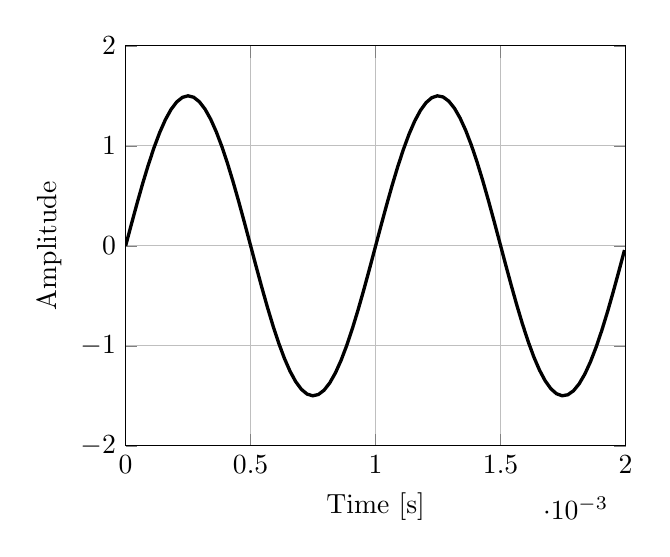
\begin{tikzpicture}

\begin{axis}[%
width=2.5in,
height=2in,
at={(1.011in,0.642in)},
scale only axis,
xmin=0,
xmax=0.002,
xlabel={Time [s]},
xmajorgrids,
ymin=-2,
ymax=2,
ylabel={Amplitude},
ymajorgrids,
axis background/.style={fill=white}
]
\addplot [color=black,solid,line width=1.2pt,forget plot]
  table[row sep=crcr]{%
0	0\\
2.26757369614512e-05	0.21299147693644\\
4.53514739229025e-05	0.421666669997482\\
6.80272108843537e-05	0.621796765035443\\
9.0702947845805e-05	0.809326114779272\\
0.000113378684807256	0.98045442674729\\
0.000136054421768707	1.13171377638122\\
0.000158730158730159	1.26003888472616\\
0.00018140589569161	1.36282923647545\\
0.000204081632653061	1.43800177955499\\
0.000226757369614512	1.48403313828686\\
0.000249433106575964	1.49999048468041\\
0.000272108843537415	1.48555044224226\\
0.000294784580498866	1.44100563921852\\
0.000317460317460317	1.36725877846751\\
0.000340136054421769	1.26580434413712\\
0.00036281179138322	1.13869831586227\\
0.000385487528344671	0.988516504225587\\
0.000408163265306122	0.818302351815823\\
0.000430839002267574	0.631505257698036\\
0.000453514739229025	0.431910675153779\\
0.000476190476190476	0.223563399264262\\
0.000498866213151927	0.0106855989178377\\
0.000521541950113379	-0.202408745672383\\
0.00054421768707483	-0.411401266012395\\
0.000566893424036281	-0.612056717299934\\
0.000589569160997732	-0.800308805890951\\
0.000612244897959184	-0.972342592961682\\
0.000634920634920635	-1.1246718044516\\
0.000657596371882086	-1.25420948059704\\
0.000680272108843537	-1.35833053333888\\
0.000702947845804989	-1.43492494387492\\
0.00072562358276644	-1.48244052230586\\
0.000748299319727891	-1.49991436284804\\
0.000770975056689342	-1.48699235717159\\
0.000793650793650794	-1.44393637042502\\
0.000816326530612245	-1.37161893452372\\
0.000839002267573696	-1.2715055662432\\
0.000861678004535147	-1.14562506844185\\
0.000884353741496599	-0.996528416260569\\
0.00090702947845805	-0.827237061472641\\
0.000929705215419501	-0.641181702599088\\
0.000952380952380952	-0.442132761616357\\
0.000975056689342404	-0.234123976149712\\
0.000997732426303855	-0.0213706555606557\\
0.00102040816326531	0.191815742526759\\
0.00104308390022676	0.401114984149397\\
0.00106575963718821	0.602285608781499\\
0.00108843537414966	0.791250882763146\\
0.00111111111111111	0.964181414529808\\
0.00113378684807256	1.11757275744087\\
0.00115646258503401	1.24831642758161\\
0.00117913832199546	1.35376289735891\\
0.00120181405895692	1.43177528832223\\
0.00122448979591837	1.48077267512167\\
0.00124716553287982	1.49976212304635\\
0.00126984126984127	1.48835880990026\\
0.00129251700680272	1.44679382444511\\
0.00131519274376417	1.37590948337396\\
0.00133786848072562	1.27714226171757\\
0.00136054421768707	1.15249368259969\\
0.00138321995464853	1.00448975626204\\
0.00140589569160998	0.836129790329203\\
0.00142857142857143	0.650825608676338\\
0.00145124716553288	0.452332410632626\\
0.00147392290249433	0.244672671662413\\
0.00149659863945578	0.0320546276809519\\
0.00151927437641723	-0.181213005075519\\
0.00154195011337868	-0.390808346418877\\
0.00156462585034014	-0.592483935346407\\
0.00158730158730159	-0.782152805069245\\
0.00160997732426304	-0.955971305616867\\
0.00163265306122449	-1.11041699561297\\
0.00165532879818594	-1.24236002474175\\
0.00167800453514739	-1.34912656033491\\
0.00170068027210884	-1.42855297273628\\
0.00172335600907029	-1.47902968137455\\
0.00174603174603175	-1.49953377300122\\
0.0017687074829932	-1.48964973108323\\
0.00179138321995465	-1.44957785626813\\
0.0018140589569161	-1.38013020728057\\
0.00183673469387755	-1.28271414450802\\
0.001859410430839	-1.15930380976591\\
0.00188208616780045	-1.01240012020625\\
0.0019047619047619	-0.844980087095434\\
0.00192743764172336	-0.660436486518814\\
0.00195011337868481	-0.462509104588652\\
0.00197278911564626	-0.25520895047495\\
0.00199546485260771	-0.0427369730862695\\
};
\end{axis}
\end{tikzpicture}%
	\caption{A 1 kHz sinusoid with a peak amplitude of 1.5.}
	\label{fig:clippingClean}
\end{subfigure}
\begin{subfigure}[t]{0.47\textwidth}
	\tikzsetnextfilename{clippingDist}
	% This file was created by matlab2tikz.
%
%The latest updates can be retrieved from
%  http://www.mathworks.com/matlabcentral/fileexchange/22022-matlab2tikz-matlab2tikz
%where you can also make suggestions and rate matlab2tikz.
%
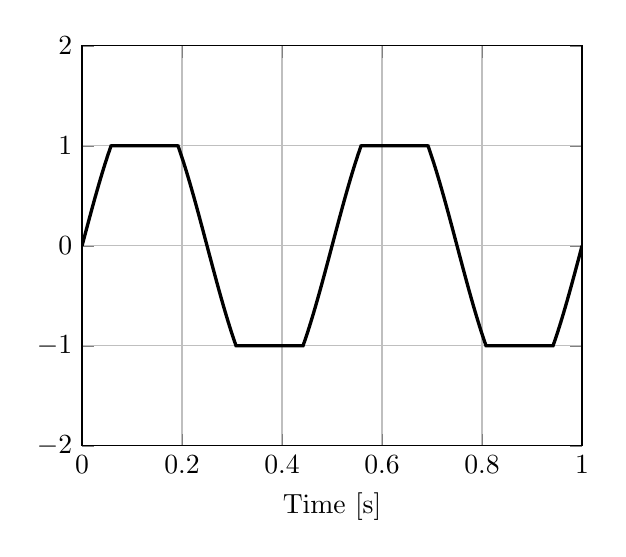
\begin{tikzpicture}

\begin{axis}[%
width=2.5in,
height=2in,
at={(1.011in,0.642in)},
scale only axis,
xmin=0,
xmax=1,
xlabel={Time [s]},
xmajorgrids,
ymin=-2,
ymax=2,
ymajorgrids,
axis background/.style={fill=white}
]
\addplot [color=black,solid,line width=1.2pt,forget plot]
  table[row sep=crcr]{%
0	0\\
0.001	0.0188490598250289\\
0.002	0.0376951431650062\\
0.003	0.0565352740049018\\
0.004	0.0753664772696543\\
0.005	0.0941857792939701\\
0.006	0.112990208291899\\
0.007	0.131776794826115\\
0.008	0.150542572276822\\
0.009	0.169284577310223\\
0.01	0.187999850346456\\
0.011	0.206685436026957\\
0.012	0.225338383681136\\
0.013	0.243955747792325\\
0.014	0.262534588462914\\
0.015	0.281071971878587\\
0.016	0.299564970771611\\
0.017	0.318010664883082\\
0.018	0.336406141424072\\
0.019	0.354748495535587\\
0.02	0.373034830747282\\
0.021	0.391262259434845\\
0.022	0.409427903275988\\
0.023	0.427528893704964\\
0.024	0.445562372365552\\
0.025	0.463525491562421\\
0.026	0.481415414710814\\
0.027	0.49922931678448\\
0.028	0.516964384761776\\
0.029	0.534617818069876\\
0.03	0.552186829027017\\
0.031	0.569668643282702\\
0.032	0.587060500255804\\
0.033	0.604359653570494\\
0.034	0.621563371489926\\
0.035	0.638668937347609\\
0.036	0.655673649976399\\
0.037	0.672574824135048\\
0.038	0.689369790932232\\
0.039	0.706055898247999\\
0.04	0.722630511152573\\
0.041	0.739091012322437\\
0.042	0.755434802453641\\
0.043	0.77165930067226\\
0.044	0.787761944941943\\
0.045	0.803740192468495\\
0.046	0.819591520101404\\
0.047	0.835313424732282\\
0.048	0.850903423690135\\
0.049	0.866359055133401\\
0.05	0.88167787843871\\
0.051	0.896857474586278\\
0.052	0.911895446541908\\
0.053	0.926789419635502\\
0.054	0.941537041936051\\
0.055	0.956135984623034\\
0.056	0.970583942354166\\
0.057	0.984878633629435\\
0.058	0.999017801151378\\
0.059	1\\
0.06	1\\
0.061	1\\
0.062	1\\
0.063	1\\
0.064	1\\
0.065	1\\
0.066	1\\
0.067	1\\
0.068	1\\
0.069	1\\
0.07	1\\
0.071	1\\
0.072	1\\
0.073	1\\
0.074	1\\
0.075	1\\
0.076	1\\
0.077	1\\
0.078	1\\
0.079	1\\
0.08	1\\
0.081	1\\
0.082	1\\
0.083	1\\
0.084	1\\
0.085	1\\
0.086	1\\
0.087	1\\
0.088	1\\
0.089	1\\
0.09	1\\
0.091	1\\
0.092	1\\
0.093	1\\
0.094	1\\
0.095	1\\
0.096	1\\
0.097	1\\
0.098	1\\
0.099	1\\
0.1	1\\
0.101	1\\
0.102	1\\
0.103	1\\
0.104	1\\
0.105	1\\
0.106	1\\
0.107	1\\
0.108	1\\
0.109	1\\
0.11	1\\
0.111	1\\
0.112	1\\
0.113	1\\
0.114	1\\
0.115	1\\
0.116	1\\
0.117	1\\
0.118	1\\
0.119	1\\
0.12	1\\
0.121	1\\
0.122	1\\
0.123	1\\
0.124	1\\
0.125	1\\
0.126	1\\
0.127	1\\
0.128	1\\
0.129	1\\
0.13	1\\
0.131	1\\
0.132	1\\
0.133	1\\
0.134	1\\
0.135	1\\
0.136	1\\
0.137	1\\
0.138	1\\
0.139	1\\
0.14	1\\
0.141	1\\
0.142	1\\
0.143	1\\
0.144	1\\
0.145	1\\
0.146	1\\
0.147	1\\
0.148	1\\
0.149	1\\
0.15	1\\
0.151	1\\
0.152	1\\
0.153	1\\
0.154	1\\
0.155	1\\
0.156	1\\
0.157	1\\
0.158	1\\
0.159	1\\
0.16	1\\
0.161	1\\
0.162	1\\
0.163	1\\
0.164	1\\
0.165	1\\
0.166	1\\
0.167	1\\
0.168	1\\
0.169	1\\
0.17	1\\
0.171	1\\
0.172	1\\
0.173	1\\
0.174	1\\
0.175	1\\
0.176	1\\
0.177	1\\
0.178	1\\
0.179	1\\
0.18	1\\
0.181	1\\
0.182	1\\
0.183	1\\
0.184	1\\
0.185	1\\
0.186	1\\
0.187	1\\
0.188	1\\
0.189	1\\
0.19	1\\
0.191	1\\
0.192	0.999017801151378\\
0.193	0.984878633629435\\
0.194	0.970583942354166\\
0.195	0.956135984623035\\
0.196	0.941537041936051\\
0.197	0.926789419635502\\
0.198	0.911895446541908\\
0.199	0.896857474586278\\
0.2	0.88167787843871\\
0.201	0.866359055133402\\
0.202	0.850903423690135\\
0.203	0.835313424732282\\
0.204	0.819591520101404\\
0.205	0.803740192468495\\
0.206	0.787761944941943\\
0.207	0.771659300672259\\
0.208	0.755434802453641\\
0.209	0.739091012322437\\
0.21	0.722630511152573\\
0.211	0.706055898247999\\
0.212	0.689369790932232\\
0.213	0.672574824135048\\
0.214	0.655673649976399\\
0.215	0.638668937347609\\
0.216	0.621563371489926\\
0.217	0.604359653570494\\
0.218	0.587060500255804\\
0.219	0.569668643282702\\
0.22	0.552186829027017\\
0.221	0.534617818069876\\
0.222	0.516964384761776\\
0.223	0.49922931678448\\
0.224	0.481415414710815\\
0.225	0.463525491562421\\
0.226	0.445562372365552\\
0.227	0.427528893704964\\
0.228	0.409427903275988\\
0.229	0.391262259434846\\
0.23	0.373034830747282\\
0.231	0.354748495535587\\
0.232	0.336406141424071\\
0.233	0.318010664883082\\
0.234	0.299564970771611\\
0.235	0.281071971878587\\
0.236	0.262534588462914\\
0.237	0.243955747792325\\
0.238	0.225338383681136\\
0.239	0.206685436026957\\
0.24	0.187999850346457\\
0.241	0.169284577310223\\
0.242	0.150542572276822\\
0.243	0.131776794826115\\
0.244	0.1129902082919\\
0.245	0.0941857792939704\\
0.246	0.0753664772696545\\
0.247	0.0565352740049018\\
0.248	0.0376951431650067\\
0.249	0.0188490598250293\\
0.25	1.83697019872103e-16\\
0.251	-0.0188490598250289\\
0.252	-0.0376951431650064\\
0.253	-0.0565352740049014\\
0.254	-0.0753664772696541\\
0.255	-0.09418577929397\\
0.256	-0.112990208291899\\
0.257	-0.131776794826114\\
0.258	-0.150542572276822\\
0.259	-0.169284577310222\\
0.26	-0.187999850346456\\
0.261	-0.206685436026957\\
0.262	-0.225338383681135\\
0.263	-0.243955747792325\\
0.264	-0.262534588462914\\
0.265	-0.281071971878587\\
0.266	-0.299564970771611\\
0.267	-0.318010664883082\\
0.268	-0.336406141424072\\
0.269	-0.354748495535587\\
0.27	-0.373034830747282\\
0.271	-0.391262259434845\\
0.272	-0.409427903275988\\
0.273	-0.427528893704964\\
0.274	-0.445562372365553\\
0.275	-0.463525491562422\\
0.276	-0.481415414710814\\
0.277	-0.49922931678448\\
0.278	-0.516964384761776\\
0.279	-0.534617818069876\\
0.28	-0.552186829027017\\
0.281	-0.569668643282702\\
0.282	-0.587060500255804\\
0.283	-0.604359653570494\\
0.284	-0.621563371489927\\
0.285	-0.638668937347609\\
0.286	-0.6556736499764\\
0.287	-0.672574824135049\\
0.288	-0.689369790932232\\
0.289	-0.706055898247998\\
0.29	-0.722630511152572\\
0.291	-0.739091012322437\\
0.292	-0.755434802453641\\
0.293	-0.771659300672259\\
0.294	-0.787761944941943\\
0.295	-0.803740192468495\\
0.296	-0.819591520101403\\
0.297	-0.835313424732281\\
0.298	-0.850903423690134\\
0.299	-0.866359055133401\\
0.3	-0.88167787843871\\
0.301	-0.896857474586278\\
0.302	-0.911895446541908\\
0.303	-0.926789419635501\\
0.304	-0.94153704193605\\
0.305	-0.956135984623034\\
0.306	-0.970583942354166\\
0.307	-0.984878633629434\\
0.308	-0.999017801151377\\
0.309	-1\\
0.31	-1\\
0.311	-1\\
0.312	-1\\
0.313	-1\\
0.314	-1\\
0.315	-1\\
0.316	-1\\
0.317	-1\\
0.318	-1\\
0.319	-1\\
0.32	-1\\
0.321	-1\\
0.322	-1\\
0.323	-1\\
0.324	-1\\
0.325	-1\\
0.326	-1\\
0.327	-1\\
0.328	-1\\
0.329	-1\\
0.33	-1\\
0.331	-1\\
0.332	-1\\
0.333	-1\\
0.334	-1\\
0.335	-1\\
0.336	-1\\
0.337	-1\\
0.338	-1\\
0.339	-1\\
0.34	-1\\
0.341	-1\\
0.342	-1\\
0.343	-1\\
0.344	-1\\
0.345	-1\\
0.346	-1\\
0.347	-1\\
0.348	-1\\
0.349	-1\\
0.35	-1\\
0.351	-1\\
0.352	-1\\
0.353	-1\\
0.354	-1\\
0.355	-1\\
0.356	-1\\
0.357	-1\\
0.358	-1\\
0.359	-1\\
0.36	-1\\
0.361	-1\\
0.362	-1\\
0.363	-1\\
0.364	-1\\
0.365	-1\\
0.366	-1\\
0.367	-1\\
0.368	-1\\
0.369	-1\\
0.37	-1\\
0.371	-1\\
0.372	-1\\
0.373	-1\\
0.374	-1\\
0.375	-1\\
0.376	-1\\
0.377	-1\\
0.378	-1\\
0.379	-1\\
0.38	-1\\
0.381	-1\\
0.382	-1\\
0.383	-1\\
0.384	-1\\
0.385	-1\\
0.386	-1\\
0.387	-1\\
0.388	-1\\
0.389	-1\\
0.39	-1\\
0.391	-1\\
0.392	-1\\
0.393	-1\\
0.394	-1\\
0.395	-1\\
0.396	-1\\
0.397	-1\\
0.398	-1\\
0.399	-1\\
0.4	-1\\
0.401	-1\\
0.402	-1\\
0.403	-1\\
0.404	-1\\
0.405	-1\\
0.406	-1\\
0.407	-1\\
0.408	-1\\
0.409	-1\\
0.41	-1\\
0.411	-1\\
0.412	-1\\
0.413	-1\\
0.414	-1\\
0.415	-1\\
0.416	-1\\
0.417	-1\\
0.418	-1\\
0.419	-1\\
0.42	-1\\
0.421	-1\\
0.422	-1\\
0.423	-1\\
0.424	-1\\
0.425	-1\\
0.426	-1\\
0.427	-1\\
0.428	-1\\
0.429	-1\\
0.43	-1\\
0.431	-1\\
0.432	-1\\
0.433	-1\\
0.434	-1\\
0.435	-1\\
0.436	-1\\
0.437	-1\\
0.438	-1\\
0.439	-1\\
0.44	-1\\
0.441	-1\\
0.442	-0.999017801151378\\
0.443	-0.984878633629435\\
0.444	-0.970583942354166\\
0.445	-0.956135984623034\\
0.446	-0.94153704193605\\
0.447	-0.926789419635502\\
0.448	-0.911895446541909\\
0.449	-0.896857474586279\\
0.45	-0.88167787843871\\
0.451	-0.866359055133402\\
0.452	-0.850903423690135\\
0.453	-0.835313424732282\\
0.454	-0.819591520101403\\
0.455	-0.803740192468494\\
0.456	-0.787761944941943\\
0.457	-0.77165930067226\\
0.458	-0.755434802453641\\
0.459	-0.739091012322437\\
0.46	-0.722630511152573\\
0.461	-0.706055898247999\\
0.462	-0.689369790932232\\
0.463	-0.672574824135048\\
0.464	-0.655673649976399\\
0.465	-0.638668937347608\\
0.466	-0.621563371489927\\
0.467	-0.604359653570494\\
0.468	-0.587060500255804\\
0.469	-0.569668643282702\\
0.47	-0.552186829027017\\
0.471	-0.534617818069876\\
0.472	-0.516964384761775\\
0.473	-0.499229316784479\\
0.474	-0.481415414710814\\
0.475	-0.463525491562421\\
0.476	-0.445562372365553\\
0.477	-0.427528893704964\\
0.478	-0.409427903275988\\
0.479	-0.391262259434845\\
0.48	-0.373034830747283\\
0.481	-0.354748495535588\\
0.482	-0.336406141424072\\
0.483	-0.318010664883082\\
0.484	-0.299564970771611\\
0.485	-0.281071971878587\\
0.486	-0.262534588462914\\
0.487	-0.243955747792326\\
0.488	-0.225338383681137\\
0.489	-0.206685436026958\\
0.49	-0.187999850346457\\
0.491	-0.169284577310223\\
0.492	-0.150542572276823\\
0.493	-0.131776794826115\\
0.494	-0.112990208291899\\
0.495	-0.0941857792939699\\
0.496	-0.0753664772696553\\
0.497	-0.0565352740049027\\
0.498	-0.0376951431650069\\
0.499	-0.0188490598250294\\
0.5	-3.67394039744206e-16\\
0.501	0.0188490598250287\\
0.502	0.0376951431650062\\
0.503	0.0565352740049019\\
0.504	0.0753664772696546\\
0.505	0.0941857792939692\\
0.506	0.112990208291898\\
0.507	0.131776794826114\\
0.508	0.150542572276822\\
0.509	0.169284577310222\\
0.51	0.187999850346456\\
0.511	0.206685436026957\\
0.512	0.225338383681136\\
0.513	0.243955747792326\\
0.514	0.262534588462913\\
0.515	0.281071971878586\\
0.516	0.29956497077161\\
0.517	0.318010664883082\\
0.518	0.336406141424072\\
0.519	0.354748495535587\\
0.52	0.373034830747282\\
0.521	0.391262259434843\\
0.522	0.409427903275988\\
0.523	0.427528893704962\\
0.524	0.445562372365552\\
0.525	0.46352549156242\\
0.526	0.481415414710814\\
0.527	0.499229316784479\\
0.528	0.516964384761776\\
0.529	0.534617818069874\\
0.53	0.552186829027017\\
0.531	0.5696686432827\\
0.532	0.587060500255804\\
0.533	0.604359653570492\\
0.534	0.621563371489926\\
0.535	0.638668937347608\\
0.536	0.655673649976399\\
0.537	0.672574824135046\\
0.538	0.689369790932232\\
0.539	0.706055898247997\\
0.54	0.722630511152573\\
0.541	0.739091012322436\\
0.542	0.755434802453641\\
0.543	0.771659300672258\\
0.544	0.787761944941944\\
0.545	0.803740192468494\\
0.546	0.819591520101404\\
0.547	0.83531342473228\\
0.548	0.850903423690135\\
0.549	0.8663590551334\\
0.55	0.88167787843871\\
0.551	0.896857474586277\\
0.552	0.911895446541908\\
0.553	0.9267894196355\\
0.554	0.941537041936051\\
0.555	0.956135984623034\\
0.556	0.970583942354167\\
0.557	0.984878633629433\\
0.558	0.999017801151378\\
0.559	1\\
0.56	1\\
0.561	1\\
0.562	1\\
0.563	1\\
0.564	1\\
0.565	1\\
0.566	1\\
0.567	1\\
0.568	1\\
0.569	1\\
0.57	1\\
0.571	1\\
0.572	1\\
0.573	1\\
0.574	1\\
0.575	1\\
0.576	1\\
0.577	1\\
0.578	1\\
0.579	1\\
0.58	1\\
0.581	1\\
0.582	1\\
0.583	1\\
0.584	1\\
0.585	1\\
0.586	1\\
0.587	1\\
0.588	1\\
0.589	1\\
0.59	1\\
0.591	1\\
0.592	1\\
0.593	1\\
0.594	1\\
0.595	1\\
0.596	1\\
0.597	1\\
0.598	1\\
0.599	1\\
0.6	1\\
0.601	1\\
0.602	1\\
0.603	1\\
0.604	1\\
0.605	1\\
0.606	1\\
0.607	1\\
0.608	1\\
0.609	1\\
0.61	1\\
0.611	1\\
0.612	1\\
0.613	1\\
0.614	1\\
0.615	1\\
0.616	1\\
0.617	1\\
0.618	1\\
0.619	1\\
0.62	1\\
0.621	1\\
0.622	1\\
0.623	1\\
0.624	1\\
0.625	1\\
0.626	1\\
0.627	1\\
0.628	1\\
0.629	1\\
0.63	1\\
0.631	1\\
0.632	1\\
0.633	1\\
0.634	1\\
0.635	1\\
0.636	1\\
0.637	1\\
0.638	1\\
0.639	1\\
0.64	1\\
0.641	1\\
0.642	1\\
0.643	1\\
0.644	1\\
0.645	1\\
0.646	1\\
0.647	1\\
0.648	1\\
0.649	1\\
0.65	1\\
0.651	1\\
0.652	1\\
0.653	1\\
0.654	1\\
0.655	1\\
0.656	1\\
0.657	1\\
0.658	1\\
0.659	1\\
0.66	1\\
0.661	1\\
0.662	1\\
0.663	1\\
0.664	1\\
0.665	1\\
0.666	1\\
0.667	1\\
0.668	1\\
0.669	1\\
0.67	1\\
0.671	1\\
0.672	1\\
0.673	1\\
0.674	1\\
0.675	1\\
0.676	1\\
0.677	1\\
0.678	1\\
0.679	1\\
0.68	1\\
0.681	1\\
0.682	1\\
0.683	1\\
0.684	1\\
0.685	1\\
0.686	1\\
0.687	1\\
0.688	1\\
0.689	1\\
0.69	1\\
0.691	1\\
0.692	0.999017801151379\\
0.693	0.984878633629435\\
0.694	0.970583942354168\\
0.695	0.956135984623035\\
0.696	0.941537041936052\\
0.697	0.926789419635501\\
0.698	0.911895446541909\\
0.699	0.896857474586278\\
0.7	0.88167787843871\\
0.701	0.866359055133401\\
0.702	0.850903423690135\\
0.703	0.835313424732281\\
0.704	0.819591520101406\\
0.705	0.803740192468493\\
0.706	0.787761944941945\\
0.707	0.771659300672258\\
0.708	0.755434802453643\\
0.709	0.739091012322438\\
0.71	0.722630511152574\\
0.711	0.706055898247999\\
0.712	0.689369790932233\\
0.713	0.672574824135051\\
0.714	0.6556736499764\\
0.715	0.638668937347611\\
0.716	0.621563371489927\\
0.717	0.604359653570496\\
0.718	0.587060500255804\\
0.719	0.569668643282703\\
0.72	0.552186829027017\\
0.721	0.534617818069877\\
0.722	0.516964384761775\\
0.723	0.499229316784481\\
0.724	0.481415414710816\\
0.725	0.463525491562422\\
0.726	0.445562372365554\\
0.727	0.427528893704964\\
0.728	0.409427903275989\\
0.729	0.391262259434845\\
0.73	0.373034830747283\\
0.731	0.354748495535587\\
0.732	0.336406141424072\\
0.733	0.318010664883084\\
0.734	0.299564970771611\\
0.735	0.281071971878589\\
0.736	0.262534588462914\\
0.737	0.243955747792327\\
0.738	0.225338383681135\\
0.739	0.206685436026958\\
0.74	0.187999850346456\\
0.741	0.169284577310223\\
0.742	0.150542572276824\\
0.743	0.131776794826115\\
0.744	0.112990208291901\\
0.745	0.0941857792939701\\
0.746	0.0753664772696555\\
0.747	0.0565352740049015\\
0.748	0.0376951431650071\\
0.749	0.0188490598250283\\
0.75	5.51091059616309e-16\\
0.751	-0.0188490598250272\\
0.752	-0.037695143165006\\
0.753	-0.0565352740049004\\
0.754	-0.0753664772696544\\
0.755	-0.094185779293969\\
0.756	-0.112990208291899\\
0.757	-0.131776794826114\\
0.758	-0.150542572276823\\
0.759	-0.169284577310222\\
0.76	-0.187999850346455\\
0.761	-0.206685436026957\\
0.762	-0.225338383681134\\
0.763	-0.243955747792326\\
0.764	-0.262534588462913\\
0.765	-0.281071971878587\\
0.766	-0.29956497077161\\
0.767	-0.318010664883083\\
0.768	-0.336406141424071\\
0.769	-0.354748495535586\\
0.77	-0.373034830747282\\
0.771	-0.391262259434844\\
0.772	-0.409427903275988\\
0.773	-0.427528893704963\\
0.774	-0.445562372365553\\
0.775	-0.463525491562421\\
0.776	-0.481415414710815\\
0.777	-0.49922931678448\\
0.778	-0.516964384761774\\
0.779	-0.534617818069876\\
0.78	-0.552186829027016\\
0.781	-0.569668643282702\\
0.782	-0.587060500255803\\
0.783	-0.604359653570495\\
0.784	-0.621563371489926\\
0.785	-0.63866893734761\\
0.786	-0.655673649976399\\
0.787	-0.67257482413505\\
0.788	-0.689369790932232\\
0.789	-0.706055898247998\\
0.79	-0.722630511152573\\
0.791	-0.739091012322437\\
0.792	-0.755434802453642\\
0.793	-0.771659300672257\\
0.794	-0.787761944941945\\
0.795	-0.803740192468493\\
0.796	-0.819591520101405\\
0.797	-0.83531342473228\\
0.798	-0.850903423690134\\
0.799	-0.8663590551334\\
0.8	-0.881677878438709\\
0.801	-0.896857474586277\\
0.802	-0.911895446541908\\
0.803	-0.9267894196355\\
0.804	-0.941537041936051\\
0.805	-0.956135984623034\\
0.806	-0.970583942354167\\
0.807	-0.984878633629434\\
0.808	-0.999017801151378\\
0.809	-1\\
0.81	-1\\
0.811	-1\\
0.812	-1\\
0.813	-1\\
0.814	-1\\
0.815	-1\\
0.816	-1\\
0.817	-1\\
0.818	-1\\
0.819	-1\\
0.82	-1\\
0.821	-1\\
0.822	-1\\
0.823	-1\\
0.824	-1\\
0.825	-1\\
0.826	-1\\
0.827	-1\\
0.828	-1\\
0.829	-1\\
0.83	-1\\
0.831	-1\\
0.832	-1\\
0.833	-1\\
0.834	-1\\
0.835	-1\\
0.836	-1\\
0.837	-1\\
0.838	-1\\
0.839	-1\\
0.84	-1\\
0.841	-1\\
0.842	-1\\
0.843	-1\\
0.844	-1\\
0.845	-1\\
0.846	-1\\
0.847	-1\\
0.848	-1\\
0.849	-1\\
0.85	-1\\
0.851	-1\\
0.852	-1\\
0.853	-1\\
0.854	-1\\
0.855	-1\\
0.856	-1\\
0.857	-1\\
0.858	-1\\
0.859	-1\\
0.86	-1\\
0.861	-1\\
0.862	-1\\
0.863	-1\\
0.864	-1\\
0.865	-1\\
0.866	-1\\
0.867	-1\\
0.868	-1\\
0.869	-1\\
0.87	-1\\
0.871	-1\\
0.872	-1\\
0.873	-1\\
0.874	-1\\
0.875	-1\\
0.876	-1\\
0.877	-1\\
0.878	-1\\
0.879	-1\\
0.88	-1\\
0.881	-1\\
0.882	-1\\
0.883	-1\\
0.884	-1\\
0.885	-1\\
0.886	-1\\
0.887	-1\\
0.888	-1\\
0.889	-1\\
0.89	-1\\
0.891	-1\\
0.892	-1\\
0.893	-1\\
0.894	-1\\
0.895	-1\\
0.896	-1\\
0.897	-1\\
0.898	-1\\
0.899	-1\\
0.9	-1\\
0.901	-1\\
0.902	-1\\
0.903	-1\\
0.904	-1\\
0.905	-1\\
0.906	-1\\
0.907	-1\\
0.908	-1\\
0.909	-1\\
0.91	-1\\
0.911	-1\\
0.912	-1\\
0.913	-1\\
0.914	-1\\
0.915	-1\\
0.916	-1\\
0.917	-1\\
0.918	-1\\
0.919	-1\\
0.92	-1\\
0.921	-1\\
0.922	-1\\
0.923	-1\\
0.924	-1\\
0.925	-1\\
0.926	-1\\
0.927	-1\\
0.928	-1\\
0.929	-1\\
0.93	-1\\
0.931	-1\\
0.932	-1\\
0.933	-1\\
0.934	-1\\
0.935	-1\\
0.936	-1\\
0.937	-1\\
0.938	-1\\
0.939	-1\\
0.94	-1\\
0.941	-1\\
0.942	-0.999017801151379\\
0.943	-0.984878633629435\\
0.944	-0.970583942354168\\
0.945	-0.956135984623037\\
0.946	-0.941537041936052\\
0.947	-0.926789419635504\\
0.948	-0.911895446541909\\
0.949	-0.89685747458628\\
0.95	-0.88167787843871\\
0.951	-0.866359055133403\\
0.952	-0.850903423690135\\
0.953	-0.835313424732283\\
0.954	-0.819591520101406\\
0.955	-0.803740192468496\\
0.956	-0.787761944941946\\
0.957	-0.771659300672261\\
0.958	-0.755434802453643\\
0.959	-0.739091012322438\\
0.96	-0.722630511152574\\
0.961	-0.706055898247999\\
0.962	-0.689369790932233\\
0.963	-0.672574824135051\\
0.964	-0.6556736499764\\
0.965	-0.638668937347611\\
0.966	-0.621563371489927\\
0.967	-0.604359653570496\\
0.968	-0.587060500255804\\
0.969	-0.569668643282703\\
0.97	-0.552186829027017\\
0.971	-0.534617818069877\\
0.972	-0.516964384761775\\
0.973	-0.499229316784481\\
0.974	-0.481415414710816\\
0.975	-0.463525491562422\\
0.976	-0.445562372365554\\
0.977	-0.427528893704965\\
0.978	-0.409427903275989\\
0.979	-0.391262259434845\\
0.98	-0.373034830747283\\
0.981	-0.354748495535587\\
0.982	-0.336406141424073\\
0.983	-0.318010664883084\\
0.984	-0.299564970771611\\
0.985	-0.281071971878589\\
0.986	-0.262534588462914\\
0.987	-0.243955747792327\\
0.988	-0.225338383681136\\
0.989	-0.206685436026958\\
0.99	-0.187999850346456\\
0.991	-0.169284577310223\\
0.992	-0.150542572276824\\
0.993	-0.131776794826115\\
0.994	-0.112990208291901\\
0.995	-0.0941857792939703\\
0.996	-0.0753664772696557\\
0.997	-0.0565352740049017\\
0.998	-0.0376951431650073\\
0.999	-0.0188490598250285\\
1	-7.34788079488412e-16\\
};
\end{axis}
\end{tikzpicture}%
	\caption{A 1 kHz clipped sinusoid.}
	\label{fig:clippingDist}
\end{subfigure}
\caption{The difference between a unaffected signal and a clipped signal. As the maximum output is 1, the signal is hard clipped because of the limitation.}
\label{fig:audioclipping}
\end{figure}

Hard clipping lowers the sound quality if the clipping is not intended, and should therefore be avoided. The wave distortion created by the sharp edge results in a square-wave-like signal. This creates additional uneven harmonics to the signal i.e. 3rd, 5th, 7th and 9th, which are unpleasant to listen to as explained in Appendix \ref{app:distortion}. Since the clipping creates the square-wave-like signal, the generation of the additional uneven harmonics can be described in the Fourier series of a square-wave. The Fourier series of a square-wave is given as:
\begin{align}\label{eq:fourier_series_square}
f(t) &= \frac{4}{\pi} (\sin(\omega_0 t) + \frac{1}{3}\sin(3 \omega_0 t) + \frac{1}{5}\sin(5 \omega_0 t) + \, ... \,)
\end{align}
\begin{where}
\va{$\omega_0$}{is the fundamental frequency of the square-wave.}{rad/s}\\
\end{where}

As seen in \autoref{eq:fourier_series_square}, the function of a square-wave signal consists of a fundamental frequency $\omega_0$ and uneven harmonics of $\omega_0$. This can also be shown in a spectrum analysis of the 1 kHz clipped sinusoid from \autoref{fig:audioclipping} in \autoref{fig:audioclippingFFT}.

\begin{figure}[H]
\centering
\begin{subfigure}[t]{0.47\textwidth}
	\tikzsetnextfilename{clippingCleanFFT}
	% This file was created by matlab2tikz.
%
%The latest updates can be retrieved from
%  http://www.mathworks.com/matlabcentral/fileexchange/22022-matlab2tikz-matlab2tikz
%where you can also make suggestions and rate matlab2tikz.
%
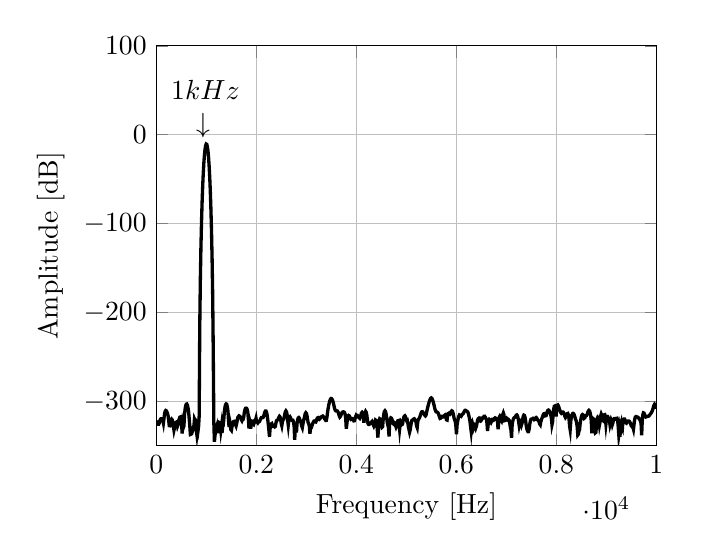
\begin{tikzpicture}

\begin{axis}[%
width=2.5in,
height=2in,
at={(1.011in,0.642in)},
scale only axis,
xmin=0,
xmax=10000,
xlabel={Frequency [Hz]},
xmajorgrids,
ymin=-350,
ymax=100,
ylabel={Amplitude [dB]},
ymajorgrids,
axis background/.style={fill=white},
]
\addplot [color=black,solid,line width=1.2pt,forget plot]
  table[row sep=crcr]{%
0	-322.11596721008\\
11.7216117216117	-323.671020481401\\
23.4432234432234	-323.340883337027\\
35.1648351648352	-325.684167070818\\
46.8864468864469	-325.669523756719\\
58.6080586080586	-324.370513022472\\
70.3296703296703	-322.159992029701\\
82.0512820512821	-319.994159311925\\
93.7728937728938	-319.483979753379\\
105.494505494505	-319.494939928451\\
117.216117216117	-320.869322942301\\
128.937728937729	-320.920572736749\\
140.659340659341	-324.227184829387\\
152.380952380952	-319.035056899834\\
164.102564102564	-313.823145631125\\
175.824175824176	-311.131574765862\\
187.545787545788	-310.246860211816\\
199.267399267399	-310.60441452423\\
210.989010989011	-311.78696455392\\
222.710622710623	-313.844752745052\\
234.432234432234	-316.418042709319\\
246.153846153846	-321.707697545501\\
257.875457875458	-327.363976836631\\
269.59706959707	-327.473089119894\\
281.318681318681	-324.112892105008\\
293.040293040293	-320.977587207666\\
304.761904761905	-319.982762533596\\
316.483516483516	-320.780760736175\\
328.205128205128	-323.668423270885\\
339.92673992674	-328.026148757277\\
351.648351648352	-332.4170697972\\
363.369963369963	-329.426095087341\\
375.091575091575	-326.556664292431\\
386.813186813187	-323.76537835188\\
398.534798534799	-323.368319264645\\
410.25641025641	-325.169104300057\\
421.978021978022	-328.189262138342\\
433.699633699634	-326.529217054039\\
445.421245421245	-322.75486943378\\
457.142857142857	-319.794087491908\\
468.864468864469	-317.719335966222\\
480.586080586081	-317.459852846429\\
492.307692307692	-319.009687543967\\
504.029304029304	-325.455766258282\\
515.750915750916	-336.106317374067\\
527.472527472527	-326.323603862667\\
539.194139194139	-329.684995875921\\
550.915750915751	-327.90212185778\\
562.637362637363	-314.792259957384\\
574.358974358974	-308.679273562794\\
586.080586080586	-304.859856763288\\
597.802197802198	-303.147924647545\\
609.52380952381	-302.958088372619\\
621.245421245421	-304.246172084633\\
632.967032967033	-307.392871145609\\
644.688644688645	-311.86240623327\\
656.410256410256	-319.720154828058\\
668.131868131868	-327.681235000644\\
679.85347985348	-337.238516322602\\
691.575091575092	-336.970257356979\\
703.296703296703	-332.332133924419\\
715.018315018315	-331.141735134048\\
726.739926739927	-332.723957001084\\
738.461538461538	-330.730504488432\\
750.18315018315	-327.778175020515\\
761.904761904762	-319.91378584982\\
773.626373626374	-321.461497849882\\
785.347985347985	-327.043537773181\\
797.069597069597	-331.841589615916\\
808.791208791209	-336.991655282628\\
820.512820512821	-330.418202230553\\
832.234432234432	-333.267393421045\\
843.956043956044	-328.226187037683\\
855.677655677656	-316.700315440438\\
867.399267399267	-215.943651772091\\
879.120879120879	-163.159584780945\\
890.842490842491	-126.529341228273\\
902.564102564103	-98.3775899142248\\
914.285714285714	-75.9321258862354\\
926.007326007326	-57.8132086793137\\
937.728937728938	-43.2219634542571\\
949.450549450549	-31.6552033180823\\
961.172161172161	-22.7812801668732\\
972.893772893773	-16.3785078578736\\
984.615384615385	-12.3020988974321\\
996.336996336996	-10.4658259320985\\
1008.05860805861	-10.8322625838136\\
1019.78021978022	-13.4088092670734\\
1031.50183150183	-18.2484666216626\\
1043.22344322344	-25.4555537550734\\
1054.94505494505	-35.1978991745999\\
1066.66666666667	-47.7291574398437\\
1078.38827838828	-63.4292414488433\\
1090.10989010989	-82.8812589369107\\
1101.8315018315	-107.032465507491\\
1113.55311355311	-137.586526131487\\
1125.27472527473	-178.243096713105\\
1136.99633699634	-241.704411925533\\
1148.71794871795	-323.195571130692\\
1160.43956043956	-345.375156099691\\
1172.16117216117	-338.247857244841\\
1183.88278388278	-333.32317434497\\
1195.6043956044	-331.269745255181\\
1207.32600732601	-328.799242404036\\
1219.04761904762	-335.934946361628\\
1230.76923076923	-327.685186138873\\
1242.49084249084	-326.960459897927\\
1254.21245421245	-323.718010447396\\
1265.93406593407	-324.108622411667\\
1277.65567765568	-326.20417623814\\
1289.37728937729	-332.697946725791\\
1301.0989010989	-327.906853738375\\
1312.82051282051	-335.418538359777\\
1324.54212454212	-328.816875760217\\
1336.26373626374	-327.262600955998\\
1347.98534798535	-320.385055874777\\
1359.70695970696	-311.475672251247\\
1371.42857142857	-306.643481149913\\
1383.15018315018	-303.695848832502\\
1394.87179487179	-302.842835407919\\
1406.59340659341	-303.232099162736\\
1418.31501831502	-305.842604461406\\
1430.03663003663	-310.40119194813\\
1441.75824175824	-320.718788147534\\
1453.47985347985	-328.69918849089\\
1465.20146520147	-321.407968983388\\
1476.92307692308	-324.473146768564\\
1488.64468864469	-331.645069484275\\
1500.3663003663	-332.515642341006\\
1512.08791208791	-328.465510911873\\
1523.80952380952	-326.826340274793\\
1535.53113553114	-324.534133776849\\
1547.25274725275	-322.615676311941\\
1558.97435897436	-322.427557967468\\
1570.69597069597	-323.530722159417\\
1582.41758241758	-326.171996895262\\
1594.13919413919	-327.712500269681\\
1605.86080586081	-325.047841087069\\
1617.58241758242	-321.24290571993\\
1629.30402930403	-317.993077517342\\
1641.02564102564	-316.998612276315\\
1652.74725274725	-316.240926477532\\
1664.46886446886	-316.68363443687\\
1676.19047619048	-317.141867195876\\
1687.91208791209	-318.342449097449\\
1699.6336996337	-320.695345632283\\
1711.35531135531	-321.836458347942\\
1723.07692307692	-320.2697737784\\
1734.79853479853	-320.163464706646\\
1746.52014652015	-317.872908059459\\
1758.24175824176	-312.6677675311\\
1769.96336996337	-309.491750132905\\
1781.68498168498	-307.828765413517\\
1793.40659340659	-307.627883691429\\
1805.12820512821	-307.890708550761\\
1816.84981684982	-309.331169961249\\
1828.57142857143	-312.28725024046\\
1840.29304029304	-320.344727197184\\
1852.01465201465	-330.483981414598\\
1863.73626373626	-320.778838487233\\
1875.45787545788	-323.188753718667\\
1887.17948717949	-330.709648822314\\
1898.9010989011	-324.458698904598\\
1910.62271062271	-322.161594474234\\
1922.34432234432	-322.355261648298\\
1934.06593406593	-325.120354775896\\
1945.78754578755	-325.813966972437\\
1957.50915750916	-323.880005799796\\
1969.23076923077	-321.560515034589\\
1980.95238095238	-321.471577902989\\
1992.67399267399	-319.02446157723\\
2004.3956043956	-323.174195056939\\
2016.11721611722	-323.174195056939\\
2027.83882783883	-324.089344868152\\
2039.56043956044	-322.910905669715\\
2051.28205128205	-323.043188327053\\
2063.00366300366	-322.552600066038\\
2074.72527472527	-320.986469744908\\
2086.44688644689	-319.545996905778\\
2098.1684981685	-318.315254794156\\
2109.89010989011	-318.387111906887\\
2121.61172161172	-318.301603114866\\
2133.33333333333	-318.177294354268\\
2145.05494505495	-316.938934301122\\
2156.77655677656	-314.354332026841\\
2168.49816849817	-312.152839226024\\
2180.21978021978	-310.876376782709\\
2191.94139194139	-310.8442203955\\
2203.663003663	-312.377716587324\\
2215.38461538462	-315.505766578087\\
2227.10622710623	-320.600055628699\\
2238.82783882784	-326.363108229676\\
2250.54945054945	-332.879313477263\\
2262.27106227106	-339.927557268938\\
2273.99267399267	-330.784134841474\\
2285.71428571429	-326.949066776775\\
2297.4358974359	-325.310562015324\\
2309.15750915751	-324.900671542525\\
2320.87912087912	-326.68176647539\\
2332.60073260073	-328.158338680386\\
2344.32234432234	-328.204122091938\\
2356.04395604396	-328.051439236523\\
2367.76556776557	-328.664204937443\\
2379.48717948718	-328.099018637999\\
2391.20879120879	-324.310047965675\\
2402.9304029304	-321.667678539627\\
2414.65201465201	-321.135207214597\\
2426.37362637363	-320.880932262159\\
2438.09523809524	-319.778960318202\\
2449.81684981685	-317.987700465117\\
2461.53846153846	-316.78808552065\\
2473.26007326007	-317.473390142408\\
2484.98168498168	-320.222893879042\\
2496.7032967033	-324.854050216358\\
2508.42490842491	-327.365492440596\\
2520.14652014652	-323.224999893465\\
2531.86813186813	-321.091227031284\\
2543.58974358974	-320.156669708411\\
2555.31135531136	-317.840663339711\\
2567.03296703297	-314.501482216247\\
2578.75457875458	-311.854837339112\\
2590.47619047619	-310.724997354159\\
2602.1978021978	-311.622091427549\\
2613.91941391941	-314.851882898182\\
2625.64102564103	-321.512762623562\\
2637.36263736264	-326.715257821487\\
2649.08424908425	-320.965390398505\\
2660.80586080586	-318.299218269644\\
2672.52747252747	-317.485994241431\\
2684.24908424908	-318.59001422949\\
2695.9706959707	-320.576544514212\\
2707.69230769231	-321.22124456977\\
2719.41391941392	-321.571973538176\\
2731.13553113553	-321.42734530042\\
2742.85714285714	-323.182504523745\\
2754.57875457875	-327.818517304439\\
2766.30036630037	-343.340028971303\\
2778.02197802198	-328.590941502845\\
2789.74358974359	-329.209198839045\\
2801.4652014652	-335.009194971263\\
2813.18681318681	-324.917874359001\\
2824.90842490842	-320.675970970006\\
2836.63003663004	-318.598485286378\\
2848.35164835165	-318.175277091238\\
2860.07326007326	-318.965978881077\\
2871.79487179487	-320.835410347703\\
2883.51648351648	-322.524929825596\\
2895.2380952381	-324.578193849772\\
2906.95970695971	-327.880455873337\\
2918.68131868132	-329.561603057853\\
2930.40293040293	-325.490736098095\\
2942.12454212454	-322.172446534305\\
2953.84615384615	-319.538366387325\\
2965.56776556777	-316.454951611266\\
2977.28937728938	-313.715712999263\\
2989.01098901099	-312.765011451191\\
3000.7326007326	-313.550082053352\\
3012.45421245421	-316.332919236015\\
3024.17582417582	-320.464673621591\\
3035.89743589744	-324.21570173302\\
3047.61904761905	-325.14025136414\\
3059.34065934066	-328.179012620665\\
3071.06227106227	-336.319390511434\\
3082.78388278388	-330.540376761589\\
3094.50549450549	-328.055385719859\\
3106.22710622711	-328.41132792291\\
3117.94871794872	-326.398110320453\\
3129.67032967033	-324.429933801343\\
3141.39194139194	-322.958523531653\\
3153.11355311355	-322.080283026816\\
3164.83516483516	-321.986069592074\\
3176.55677655678	-322.88974461944\\
3188.27838827839	-323.14866547361\\
3200	-321.731991922314\\
3211.72161172161	-319.583271135606\\
3223.44322344322	-318.524693510682\\
3235.16483516484	-318.277835267365\\
3246.88644688645	-319.493530184348\\
3258.60805860806	-320.194783095862\\
3270.32967032967	-319.645880585364\\
3282.05128205128	-318.402355114397\\
3293.77289377289	-317.597734351514\\
3305.49450549451	-317.02187364446\\
3317.21611721612	-316.763942230905\\
3328.93772893773	-316.47058612926\\
3340.65934065934	-317.197718055388\\
3352.38095238095	-318.34030296296\\
3364.10256410256	-319.71475362671\\
3375.82417582418	-320.433372545647\\
3387.54578754579	-321.481423753538\\
3399.2673992674	-321.328758210847\\
3410.98901098901	-317.848121944058\\
3422.71062271062	-312.6052633917\\
3434.43223443223	-308.209983131555\\
3446.15384615385	-304.542297484367\\
3457.87545787546	-301.476640468968\\
3469.59706959707	-299.074162567864\\
3481.31868131868	-297.505270833626\\
3493.04029304029	-296.820826693279\\
3504.7619047619	-296.952977362533\\
3516.48351648352	-297.832794363821\\
3528.20512820513	-299.532668899083\\
3539.92673992674	-301.925997253397\\
3551.64835164835	-304.833072981485\\
3563.36996336996	-307.679247836289\\
3575.09157509158	-309.820085030418\\
3586.81318681319	-310.691494738001\\
3598.5347985348	-310.817398824033\\
3610.25641025641	-310.678764468745\\
3621.97802197802	-310.904852964739\\
3633.69963369963	-312.083008289962\\
3645.42124542125	-314.044889957489\\
3657.14285714286	-316.283113404039\\
3668.86446886447	-317.725995742272\\
3680.58608058608	-316.98711432429\\
3692.30769230769	-315.404661196974\\
3704.0293040293	-313.574046253917\\
3715.75091575092	-312.403769243541\\
3727.47252747253	-311.900292301962\\
3739.19413919414	-311.790821532916\\
3750.91575091575	-311.885255334962\\
3762.63736263736	-312.507671076698\\
3774.35897435897	-314.393900840475\\
3786.08058608059	-318.958623783513\\
3797.8021978022	-330.766521534997\\
3809.52380952381	-325.502820472922\\
3821.24542124542	-319.47490837836\\
3832.96703296703	-316.5879349607\\
3844.68864468864	-315.820977290156\\
3856.41025641026	-316.165835542033\\
3868.13186813187	-317.693295629945\\
3879.85347985348	-319.724105063858\\
3891.57509157509	-320.385668853013\\
3903.2967032967	-319.982487927687\\
3915.01831501832	-319.299311012412\\
3926.73992673993	-319.444342321726\\
3938.46153846154	-320.526575483676\\
3950.18315018315	-321.926779712727\\
3961.90476190476	-321.781804018036\\
3973.62637362637	-319.294600071473\\
3985.34798534799	-317.199406352915\\
3997.0695970696	-315.48532686416\\
4008.79120879121	-316.133918462084\\
4020.51282051282	-315.922088122408\\
4032.23443223443	-316.716666209588\\
4043.95604395604	-317.865988888969\\
4055.67765567766	-318.280559925241\\
4067.39926739927	-318.926776854331\\
4079.12087912088	-317.317696380994\\
4090.84249084249	-315.060841214154\\
4102.5641025641	-312.993854282692\\
4114.28571428571	-312.27769957935\\
4126.00732600733	-313.058993411349\\
4137.72893772894	-316.497495126966\\
4149.45054945055	-324.074551114817\\
4161.17216117216	-317.815498249607\\
4172.89377289377	-312.724221795712\\
4184.61538461538	-311.184304154482\\
4196.336996337	-312.180395095067\\
4208.05860805861	-315.33167553721\\
4219.78021978022	-320.223371703619\\
4231.50183150183	-324.981894832223\\
4243.22344322344	-325.968094640368\\
4254.94505494505	-325.975199382868\\
4266.66666666667	-325.044494992807\\
4278.38827838828	-324.748701483869\\
4290.10989010989	-324.298796557654\\
4301.8315018315	-323.185408013847\\
4313.55311355311	-322.493712256323\\
4325.27472527472	-324.004517791407\\
4336.99633699634	-326.395781230683\\
4348.71794871795	-327.81152123793\\
4360.43956043956	-326.215243804676\\
4372.16117216117	-323.991135829513\\
4383.88278388278	-320.982207180012\\
4395.6043956044	-321.462465973861\\
4407.32600732601	-324.176499385288\\
4419.04761904762	-332.267280302068\\
4430.76923076923	-340.80932861649\\
4442.49084249084	-326.258684322367\\
4454.21245421245	-321.442965268777\\
4465.93406593407	-319.544444432877\\
4477.65567765568	-320.026440215285\\
4489.37728937729	-321.870034014714\\
4501.0989010989	-325.275880091975\\
4512.82051282051	-329.135133788708\\
4524.54212454212	-328.535733131409\\
4536.26373626374	-319.872005913471\\
4547.98534798535	-314.353155551714\\
4559.70695970696	-311.431276989024\\
4571.42857142857	-310.598208874572\\
4583.15018315018	-311.541465335688\\
4594.87179487179	-314.262904844306\\
4606.59340659341	-318.957659426667\\
4618.31501831502	-324.341801794823\\
4630.03663003663	-326.908025760342\\
4641.75824175824	-329.671708602847\\
4653.47985347985	-339.598374824666\\
4665.20146520146	-324.239834487312\\
4676.92307692308	-320.142812870027\\
4688.64468864469	-318.579390590904\\
4700.3663003663	-318.904551228728\\
4712.08791208791	-320.164411571421\\
4723.80952380952	-323.552244720139\\
4735.53113553114	-325.133901656344\\
4747.25274725275	-325.67494410303\\
4758.97435897436	-323.730925971029\\
4770.69597069597	-324.141194152127\\
4782.41758241758	-327.036177280335\\
4794.13919413919	-329.052455856504\\
4805.86080586081	-327.62366085932\\
4817.58241758242	-324.243757917428\\
4829.30402930403	-321.85425099731\\
4841.02564102564	-321.644312334699\\
4852.74725274725	-324.65913326885\\
4864.46886446886	-331.375490539255\\
4876.19047619048	-325.679255623113\\
4887.91208791209	-322.838347325296\\
4899.6336996337	-323.86912625874\\
4911.35531135531	-326.111153620671\\
4923.07692307692	-325.63048628826\\
4934.79853479854	-321.471648674554\\
4946.52014652015	-318.118465437495\\
4958.24175824176	-316.68211874222\\
4969.96336996337	-316.211579968543\\
4981.68498168498	-317.228440996576\\
4993.40659340659	-319.26351539118\\
5005.12820512821	-321.443807346433\\
5016.84981684982	-321.020667676622\\
5028.57142857143	-324.31969794583\\
5040.29304029304	-328.84177524509\\
5052.01465201465	-331.83382615458\\
5063.73626373626	-334.735835579055\\
5075.45787545788	-332.299258886241\\
5087.17948717949	-327.630942194737\\
5098.9010989011	-323.781987640664\\
5110.62271062271	-321.395765925455\\
5122.34432234432	-320.886447997559\\
5134.06593406593	-320.465428875501\\
5145.78754578755	-319.820250617952\\
5157.50915750916	-319.568122144542\\
5169.23076923077	-320.445377078076\\
5180.95238095238	-321.775888699888\\
5192.67399267399	-323.327196438195\\
5204.3956043956	-327.748774429116\\
5216.11721611722	-329.500414479457\\
5227.83882783883	-322.930677708616\\
5239.56043956044	-320.345390384961\\
5251.28205128205	-319.46742292498\\
5263.00366300366	-318.422700195226\\
5274.72527472528	-316.460548794413\\
5286.44688644689	-314.420570373633\\
5298.1684981685	-312.634917234304\\
5309.89010989011	-311.645830096681\\
5321.61172161172	-311.606321565998\\
5333.33333333333	-312.395026397497\\
5345.05494505495	-313.644669672522\\
5356.77655677656	-314.764393688141\\
5368.49816849817	-315.637442053714\\
5380.21978021978	-316.335135300277\\
5391.94139194139	-315.462866674828\\
5403.663003663	-312.472956024358\\
5415.38461538462	-309.49096542544\\
5427.10622710623	-306.661910098118\\
5438.82783882784	-304.082440188536\\
5450.54945054945	-301.618020574783\\
5462.27106227106	-299.473868003226\\
5473.99267399267	-297.699114290504\\
5485.71428571429	-296.505406176026\\
5497.4358974359	-296.028411377836\\
5509.15750915751	-296.481646635714\\
5520.87912087912	-297.788088059893\\
5532.60073260073	-299.767551285277\\
5544.32234432234	-302.299391403697\\
5556.04395604396	-305.019492670558\\
5567.76556776557	-307.832948492747\\
5579.48717948718	-310.176717152399\\
5591.20879120879	-311.537518356175\\
5602.9304029304	-312.01745525393\\
5614.65201465201	-312.046097429218\\
5626.37362637363	-312.503028224505\\
5638.09523809524	-313.577705423825\\
5649.81684981685	-315.357798221399\\
5661.53846153846	-317.508009492954\\
5673.26007326007	-319.196199557734\\
5684.98168498169	-318.94203762454\\
5696.7032967033	-317.879613158787\\
5708.42490842491	-316.798370316049\\
5720.14652014652	-316.82023072804\\
5731.86813186813	-317.520829533155\\
5743.58974358974	-317.470921782045\\
5755.31135531136	-316.636505065392\\
5767.03296703297	-315.48666870282\\
5778.75457875458	-315.086859657696\\
5790.47619047619	-316.558142674321\\
5802.1978021978	-320.779865087743\\
5813.91941391941	-321.054678726594\\
5825.64102564103	-316.14666429264\\
5837.36263736264	-313.693752780448\\
5849.08424908425	-313.306516635395\\
5860.80586080586	-313.996318878861\\
5872.52747252747	-314.37620671086\\
5884.24908424908	-313.166557488194\\
5895.9706959707	-311.376347149641\\
5907.69230769231	-310.609368275481\\
5919.41391941392	-311.055178949651\\
5931.13553113553	-312.880034391828\\
5942.85714285714	-315.651542934863\\
5954.57875457875	-318.878501759082\\
5966.30036630037	-321.036914294143\\
5978.02197802198	-322.640785223042\\
5989.74358974359	-327.717946996982\\
6001.4652014652	-336.905142623736\\
6013.18681318681	-327.005050138264\\
6024.90842490843	-322.811148168367\\
6036.63003663004	-319.380448937682\\
6048.35164835165	-316.788794523067\\
6060.07326007326	-315.260026736671\\
6071.79487179487	-315.500235117214\\
6083.51648351648	-316.31262723076\\
6095.2380952381	-316.737763870142\\
6106.95970695971	-315.570585456679\\
6118.68131868132	-314.512473865216\\
6130.40293040293	-314.136967184497\\
6142.12454212454	-313.29777999593\\
6153.84615384615	-311.709230965213\\
6165.56776556777	-310.49076173709\\
6177.28937728938	-310.045515193581\\
6189.01098901099	-310.246728483171\\
6200.7326007326	-310.787694641331\\
6212.45421245421	-311.176489009487\\
6224.17582417582	-311.809877276123\\
6235.89743589744	-313.113077702783\\
6247.61904761905	-315.616909829523\\
6259.34065934066	-318.661714183517\\
6271.06227106227	-322.313080483317\\
6282.78388278388	-327.918824513223\\
6294.50549450549	-333.109040304427\\
6306.22710622711	-325.927465960554\\
6317.94871794872	-323.996489833835\\
6329.67032967033	-326.273728960488\\
6341.39194139194	-330.315574560491\\
6353.11355311355	-328.483366853066\\
6364.83516483516	-326.74920929609\\
6376.55677655678	-327.49073574341\\
6388.27838827839	-329.789351229632\\
6400	-327.930813274501\\
6411.72161172161	-324.610485895231\\
6423.44322344322	-321.167986704039\\
6435.16483516484	-319.665930677914\\
6446.88644688645	-319.111410353944\\
6458.60805860806	-320.364903454833\\
6470.32967032967	-321.914877776708\\
6482.05128205128	-322.313799686604\\
6493.77289377289	-321.740312795319\\
6505.49450549451	-319.296121098251\\
6517.21611721612	-319.69294349133\\
6528.93772893773	-318.952028639534\\
6540.65934065934	-318.501704630851\\
6552.38095238095	-316.777475572032\\
6564.10256410256	-316.717006826668\\
6575.82417582418	-317.61125822692\\
6587.54578754579	-318.786507250062\\
6599.2673992674	-320.239735171892\\
6610.98901098901	-324.104041604204\\
6622.71062271062	-333.35063319449\\
6634.43223443223	-326.537528631427\\
6646.15384615385	-321.590163141839\\
6657.87545787546	-320.404503211436\\
6669.59706959707	-321.094255003877\\
6681.31868131868	-322.52941342568\\
6693.04029304029	-323.673564331662\\
6704.7619047619	-322.201692071793\\
6716.48351648352	-320.244858854374\\
6728.20512820513	-320.251901048602\\
6739.92673992674	-321.35689658538\\
6751.64835164835	-320.990179578456\\
6763.36996336996	-319.060876489788\\
6775.09157509157	-318.533942823261\\
6786.81318681319	-318.916808430597\\
6798.5347985348	-319.518804604868\\
6810.25641025641	-319.924529824657\\
6821.97802197802	-321.980145450263\\
6833.69963369963	-331.458275918032\\
6845.42124542125	-324.125151967631\\
6857.14285714286	-317.900153356718\\
6868.86446886447	-316.689697147324\\
6880.58608058608	-317.850204581596\\
6892.30769230769	-320.962901491635\\
6904.0293040293	-322.04501633756\\
6915.75091575092	-319.148423142536\\
6927.47252747253	-314.712507000867\\
6939.19413919414	-312.955201335434\\
6950.91575091575	-314.934438338139\\
6962.63736263736	-321.691805921343\\
6974.35897435897	-321.507416252971\\
6986.08058608059	-318.913831166071\\
6997.8021978022	-318.537296556117\\
7009.52380952381	-319.664940734387\\
7021.24542124542	-321.033184631024\\
7032.96703296703	-321.280597507472\\
7044.68864468864	-320.65348783344\\
7056.41025641026	-321.544268892108\\
7068.13186813187	-324.909985331434\\
7079.85347985348	-329.313186838791\\
7091.57509157509	-332.280661546479\\
7103.2967032967	-341.061236750148\\
7115.01831501831	-326.69538279765\\
7126.73992673993	-322.292835964636\\
7138.46153846154	-319.989311376396\\
7150.18315018315	-318.630002550268\\
7161.90476190476	-318.245973589254\\
7173.62637362637	-317.726642570322\\
7185.34798534799	-316.718635481522\\
7197.0695970696	-315.563757275132\\
7208.79120879121	-315.241824611678\\
7220.51282051282	-316.080440447667\\
7232.23443223443	-318.468702319092\\
7243.95604395604	-322.360684600848\\
7255.67765567766	-327.075552711074\\
7267.39926739927	-324.075922278487\\
7279.12087912088	-322.751656854546\\
7290.84249084249	-323.770874889428\\
7302.5641025641	-326.404213176727\\
7314.28571428571	-324.276513906979\\
7326.00732600733	-319.604985711716\\
7337.72893772894	-316.885227851634\\
7349.45054945055	-315.509440863834\\
7361.17216117216	-315.885980380922\\
7372.89377289377	-317.869887758875\\
7384.61538461538	-321.828379980733\\
7396.336996337	-326.972248335253\\
7408.05860805861	-330.816247724348\\
7419.78021978022	-332.917816247661\\
7431.50183150183	-334.088345139144\\
7443.22344322344	-334.039541659792\\
7454.94505494505	-331.317388375006\\
7466.66666666667	-326.042889798033\\
7478.38827838828	-322.273380544063\\
7490.10989010989	-320.228852146628\\
7501.8315018315	-319.825748766459\\
7513.55311355311	-319.857391327868\\
7525.27472527472	-319.575147399642\\
7536.99633699634	-319.002593782705\\
7548.71794871795	-319.189564887987\\
7560.43956043956	-320.595668636434\\
7572.16117216117	-320.283451105186\\
7583.88278388278	-318.747557790846\\
7595.6043956044	-318.197353454484\\
7607.32600732601	-318.710969603356\\
7619.04761904762	-320.253628300766\\
7630.76923076923	-321.304743861674\\
7642.49084249084	-321.968430414262\\
7654.21245421245	-323.049962851721\\
7665.93406593407	-325.425545473352\\
7677.65567765568	-326.342696276617\\
7689.37728937729	-322.719449251711\\
7701.0989010989	-320.46831812036\\
7712.82051282051	-318.760001458868\\
7724.54212454212	-317.09655389246\\
7736.26373626374	-315.071735053495\\
7747.98534798535	-313.957311862731\\
7759.70695970696	-313.777693147284\\
7771.42857142857	-314.758129461551\\
7783.15018315018	-316.221807584924\\
7794.87179487179	-316.004488167775\\
7806.59340659341	-313.685718324277\\
7818.31501831502	-311.394385709246\\
7830.03663003663	-310.070987426456\\
7841.75824175824	-309.752125968274\\
7853.47985347985	-310.244001457788\\
7865.20146520146	-311.377831509964\\
7876.92307692308	-313.078872034432\\
7888.64468864469	-315.500912184438\\
7900.3663003663	-319.10387215923\\
7912.08791208791	-326.28316885154\\
7923.80952380952	-323.380220502685\\
7935.53113553114	-313.448462236168\\
7947.25274725275	-308.294593683721\\
7958.97435897436	-305.469872674311\\
7970.69597069597	-305.167011673318\\
7982.41758241758	-308.634255813916\\
7994.13919413919	-316.996533610232\\
8005.86080586081	-308.12293814028\\
8017.58241758242	-304.377504025446\\
8029.30402930403	-304.020267480002\\
8041.02564102564	-305.245092704997\\
8052.74725274725	-307.106704328033\\
8064.46886446886	-309.086313498283\\
8076.19047619048	-310.96731260196\\
8087.91208791209	-312.723937148097\\
8099.6336996337	-313.40704912385\\
8111.35531135531	-312.881595411821\\
8123.07692307692	-312.00916316847\\
8134.79853479854	-312.045022818734\\
8146.52014652015	-312.891778648313\\
8158.24175824176	-314.769138299542\\
8169.96336996337	-316.926983630867\\
8181.68498168498	-318.331174630807\\
8193.40659340659	-317.523550478908\\
8205.12820512821	-315.624305125197\\
8216.84981684982	-313.889651021461\\
8228.57142857143	-313.604030730005\\
8240.29304029304	-315.182380119884\\
8252.01465201465	-319.325473656725\\
8263.73626373626	-327.749453700273\\
8275.45787545788	-331.855026378785\\
8287.17948717949	-322.62698863878\\
8298.9010989011	-318.01637616263\\
8310.62271062271	-315.208784141468\\
8322.34432234432	-313.894076468293\\
8334.06593406593	-313.503042816163\\
8345.78754578755	-313.87960482866\\
8357.50915750916	-315.224182739521\\
8369.23076923077	-317.240425254906\\
8380.95238095238	-319.736321376281\\
8392.67399267399	-321.254047539748\\
8404.3956043956	-324.010233142261\\
8416.11721611722	-328.538728115761\\
8427.83882783883	-337.823877717833\\
8439.56043956044	-336.949407077552\\
8451.28205128205	-333.118511514039\\
8463.00366300366	-332.001656723397\\
8474.72527472528	-325.501971726821\\
8486.44688644689	-320.914359167317\\
8498.1684981685	-317.66818632746\\
8509.89010989011	-315.457814733265\\
8521.61172161172	-314.795068873777\\
8533.33333333333	-315.214845207219\\
8545.05494505494	-317.202945241855\\
8556.77655677656	-319.051731115371\\
8568.49816849817	-318.525423436787\\
8580.21978021978	-316.702944103822\\
8591.94139194139	-316.0284409738\\
8603.663003663	-315.871280453112\\
8615.38461538462	-314.62653488061\\
8627.10622710623	-312.417761597356\\
8638.82783882784	-310.750449848843\\
8650.54945054945	-310.110496780526\\
8662.27106227106	-310.833812693323\\
8673.99267399267	-312.68666544051\\
8685.71428571429	-315.715177792846\\
8697.4358974359	-321.661749190294\\
8709.15750915751	-336.001939369131\\
8720.87912087912	-322.665696991299\\
8732.60073260073	-319.319101086666\\
8744.32234432235	-319.855577066449\\
8756.04395604396	-324.263179260977\\
8767.76556776557	-331.334904609174\\
8779.48717948718	-335.369866527898\\
8791.20879120879	-334.842292764466\\
8802.9304029304	-323.701618245851\\
8814.65201465201	-319.550304857543\\
8826.37362637363	-318.016762190182\\
8838.09523809524	-318.792292612452\\
8849.81684981685	-321.175445884337\\
8861.53846153846	-326.682361842261\\
8873.26007326007	-323.228724665491\\
8884.98168498169	-316.461523942199\\
8896.7032967033	-314.241802268579\\
8908.42490842491	-315.784091907295\\
8920.14652014652	-321.142336319666\\
8931.86813186813	-321.656356631991\\
8943.58974358974	-317.306846269729\\
8955.31135531135	-315.113626491219\\
8967.03296703297	-314.94291889927\\
8978.75457875458	-318.584442639277\\
8990.47619047619	-325.486387056894\\
9002.1978021978	-319.579875492852\\
9013.91941391941	-316.882558847297\\
9025.64102564103	-316.971141428778\\
9037.36263736264	-318.466398649446\\
9049.08424908425	-319.584477345085\\
9060.80586080586	-321.925033508817\\
9072.52747252747	-326.581267266232\\
9084.24908424908	-324.124995000819\\
9095.9706959707	-321.017079921336\\
9107.69230769231	-322.549984098794\\
9119.41391941392	-326.040213153238\\
9131.13553113553	-323.945724098535\\
9142.85714285714	-320.379631465688\\
9154.57875457876	-319.455386854021\\
9166.30036630037	-319.581951804999\\
9178.02197802198	-320.059608458932\\
9189.74358974359	-319.793353937548\\
9201.4652014652	-318.926337759079\\
9213.18681318681	-318.894725174424\\
9224.90842490842	-321.273469818891\\
9236.63003663004	-328.439932149163\\
9248.35164835165	-337.705103000116\\
9260.07326007326	-332.847373517492\\
9271.79487179487	-339.807028380806\\
9283.51648351648	-326.683848369415\\
9295.2380952381	-324.254373077211\\
9306.95970695971	-329.575387569113\\
9318.68131868132	-331.033092103955\\
9330.40293040293	-322.4988146288\\
9342.12454212454	-320.31694471732\\
9353.84615384615	-319.813537971468\\
9365.56776556777	-319.893520872533\\
9377.28937728938	-321.746167442506\\
9389.01098901099	-324.093065926373\\
9400.7326007326	-324.545190927801\\
9412.45421245421	-323.566290996444\\
9424.17582417582	-322.400038393721\\
9435.89743589744	-322.082696726137\\
9447.61904761905	-322.096131925715\\
9459.34065934066	-322.535337163933\\
9471.06227106227	-323.754085860336\\
9482.78388278388	-324.248515632614\\
9494.50549450549	-327.217812090358\\
9506.22710622711	-327.908856835558\\
9517.94871794872	-328.840796657921\\
9529.67032967033	-328.941622871132\\
9541.39194139194	-331.372833778235\\
9553.11355311355	-325.933039818903\\
9564.83516483517	-320.754424534769\\
9576.55677655678	-317.94285788656\\
9588.27838827839	-317.129267511687\\
9600	-317.177503142123\\
9611.72161172161	-317.483296225311\\
9623.44322344322	-317.683681640523\\
9635.16483516483	-318.053083224603\\
9646.88644688645	-318.962342883504\\
9658.60805860806	-319.591463893405\\
9670.32967032967	-320.995259679806\\
9682.05128205128	-322.148728534897\\
9693.77289377289	-325.205248015548\\
9705.49450549451	-338.292528632461\\
9717.21611721612	-321.490199903432\\
9728.93772893773	-315.133184231579\\
9740.65934065934	-312.912515642843\\
9752.38095238095	-313.154570095418\\
9764.10256410256	-314.932810553675\\
9775.82417582418	-316.957374431456\\
9787.54578754579	-317.625479724005\\
9799.2673992674	-317.279551035858\\
9810.98901098901	-316.912417510879\\
9822.71062271062	-316.855602042584\\
9834.43223443223	-316.693982290875\\
9846.15384615385	-316.614494989827\\
9857.87545787546	-315.942897473474\\
9869.59706959707	-315.102082640757\\
9881.31868131868	-314.124929042546\\
9893.04029304029	-313.198169019211\\
9904.7619047619	-312.194338273337\\
9916.48351648352	-310.828950422181\\
9928.20512820513	-308.983169376293\\
9939.92673992674	-306.598046051289\\
9951.64835164835	-304.398163642745\\
9963.36996336996	-303.254593784378\\
9975.09157509158	-304.122276065458\\
9986.81318681319	-308.43604201762\\
};
\node[right, align=left, text=black]
at (axis cs:600,10) {$\downarrow$};
\node[right, align=left, text=black]
at (axis cs:100,50) {$\text{1 kHz}$};
\end{axis}
\end{tikzpicture}%
	\caption{FFT of a 1 kHz sinusoid without clipping.}
	\label{fig:clippingCleanFFT}
\end{subfigure}
\hspace{6mm} 
\begin{subfigure}[t]{0.47\textwidth}
	\tikzsetnextfilename{clippingDistFFT}
	% This file was created by matlab2tikz.
%
%The latest updates can be retrieved from
%  http://www.mathworks.com/matlabcentral/fileexchange/22022-matlab2tikz-matlab2tikz
%where you can also make suggestions and rate matlab2tikz.
%
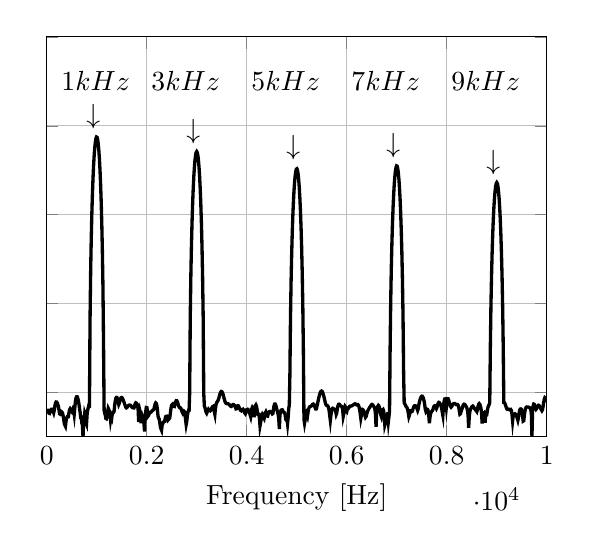
\begin{tikzpicture}

\begin{axis}[%
width=2.5in,
height=2in,
at={(1.011in,0.642in)},
scale only axis,
xmin=0,
xmax=10000,
xlabel={Frequency [Hz]},
xmajorgrids,
ymin=-350,
ymax=100,
yticklabels={\empty},
ymajorgrids,
axis background/.style={fill=white}
]
\addplot [color=black,solid,line width=1.2pt,forget plot]
  table[row sep=crcr]{%
0	-319.66977604872\\
11.7216117216117	-320.252664587285\\
23.4432234432234	-320.150235457912\\
35.1648351648352	-321.87769890753\\
46.8864468864469	-323.40415662653\\
58.6080586080586	-323.656130393623\\
70.3296703296703	-322.064437707905\\
82.0512820512821	-319.981208617154\\
93.7728937728938	-318.842227630664\\
105.494505494505	-318.824139809043\\
117.216117216117	-320.887574922404\\
128.937728937729	-321.003133041111\\
140.659340659341	-322.87596816246\\
152.380952380952	-319.992614901689\\
164.102564102564	-315.14338512313\\
175.824175824176	-312.091040412566\\
187.545787545788	-310.719044223205\\
199.267399267399	-310.809798667983\\
210.989010989011	-311.752989871661\\
222.710622710623	-313.45380396223\\
234.432234432234	-315.761867809304\\
246.153846153846	-319.502071438942\\
257.875457875458	-323.946635313474\\
269.59706959707	-324.371444723204\\
281.318681318681	-323.073351060989\\
293.040293040293	-321.551796444871\\
304.761904761905	-322.055919814239\\
316.483516483516	-322.965971780673\\
328.205128205128	-326.002185265755\\
339.92673992674	-329.965312555944\\
351.648351648352	-334.711128765065\\
363.369963369963	-336.638049322374\\
375.091575091575	-337.98571585667\\
386.813186813187	-332.646513976849\\
398.534798534799	-328.549789756313\\
410.25641025641	-327.456662133417\\
421.978021978022	-327.626158860462\\
433.699633699634	-327.386942727765\\
445.421245421245	-322.896618361246\\
457.142857142857	-319.559352515529\\
468.864468864469	-318.409730305314\\
480.586080586081	-319.522058201484\\
492.307692307692	-320.47758374283\\
504.029304029304	-321.509888136428\\
515.750915750916	-320.159719568534\\
527.472527472527	-318.379124501943\\
539.194139194139	-319.523442928177\\
550.915750915751	-324.291519604555\\
562.637362637363	-317.000247172954\\
574.358974358974	-310.257297372003\\
586.080586080586	-306.452256789241\\
597.802197802198	-304.914755096574\\
609.52380952381	-304.849950666219\\
621.245421245421	-306.178349309972\\
632.967032967033	-308.999456883321\\
644.688644688645	-312.701079748048\\
656.410256410256	-318.133369508358\\
668.131868131868	-321.871349328687\\
679.85347985348	-328.007141062136\\
691.575091575092	-327.923815494954\\
703.296703296703	-334.421366290934\\
715.018315018315	-336.919165990102\\
726.739926739927	-350.238350354447\\
738.461538461538	-334.287106214054\\
750.18315018315	-331.529493482922\\
761.904761904762	-323.393743024448\\
773.626373626374	-325.375012877451\\
785.347985347985	-333.280057572197\\
797.069597069597	-335.19416243948\\
808.791208791209	-324.722376849988\\
820.512820512821	-319.534300482415\\
832.234432234432	-317.094423031942\\
843.956043956044	-314.230543015098\\
855.677655677656	-314.557553385869\\
867.399267399267	-218.096479418237\\
879.120879120879	-165.31233950964\\
890.842490842491	-128.682095822832\\
902.564102564103	-100.530344507165\\
914.285714285714	-78.084880479123\\
926.007326007326	-59.9659632721987\\
937.728937728938	-45.374718047142\\
949.450549450549	-33.8079579109673\\
961.172161172161	-24.9340347597582\\
972.893772893773	-18.5312624507586\\
984.615384615385	-14.4548534903171\\
996.336996336996	-12.6185805249835\\
1008.05860805861	-12.9850171766986\\
1019.78021978022	-15.5615638599584\\
1031.50183150183	-20.4012212145476\\
1043.22344322344	-27.6083083479584\\
1054.94505494505	-37.3506537674849\\
1066.66666666667	-49.8819120327287\\
1078.38827838828	-65.5819960417282\\
1090.10989010989	-85.0340135297919\\
1101.8315018315	-109.185220100279\\
1113.55311355311	-139.739280721206\\
1125.27472527473	-180.395851142773\\
1136.99633699634	-243.857203771645\\
1148.71794871795	-320.064214921221\\
1160.43956043956	-323.366413363497\\
1172.16117216117	-325.396412628388\\
1183.88278388278	-329.265224803788\\
1195.6043956044	-329.60094243683\\
1207.32600732601	-326.921780096168\\
1219.04761904762	-321.464324984819\\
1230.76923076923	-317.826268547569\\
1242.49084249084	-319.221077345555\\
1254.21245421245	-321.375095535668\\
1265.93406593407	-324.721808786549\\
1277.65567765568	-331.172690405964\\
1289.37728937729	-327.190232156617\\
1301.0989010989	-328.859943718811\\
1312.82051282051	-323.934795224629\\
1324.54212454212	-322.364415478264\\
1336.26373626374	-322.478330039218\\
1347.98534798535	-321.489536953464\\
1359.70695970696	-314.390389588376\\
1371.42857142857	-309.60862386725\\
1383.15018315018	-306.521750201537\\
1394.87179487179	-305.565117533603\\
1406.59340659341	-305.702100348221\\
1418.31501831502	-307.818779142851\\
1430.03663003663	-310.811026454631\\
1441.75824175824	-313.559439282394\\
1453.47985347985	-312.058365319402\\
1465.20146520147	-309.48643321096\\
1476.92307692308	-307.140766755864\\
1488.64468864469	-305.927929790195\\
1500.3663003663	-305.68081936221\\
1512.08791208791	-306.253463667057\\
1523.80952380952	-307.512548043642\\
1535.53113553114	-309.240333775713\\
1547.25274725275	-311.110810007732\\
1558.97435897436	-313.026613238936\\
1570.69597069597	-314.684246329279\\
1582.41758241758	-316.562263550235\\
1594.13919413919	-317.34925468497\\
1605.86080586081	-316.972914787236\\
1617.58241758242	-315.837162513633\\
1629.30402930403	-315.010289548155\\
1641.02564102564	-314.61272550257\\
1652.74725274725	-314.191796909467\\
1664.46886446886	-314.28452593732\\
1676.19047619048	-314.44068736787\\
1687.91208791209	-315.163984330929\\
1699.6336996337	-316.074197397418\\
1711.35531135531	-316.88489131864\\
1723.07692307692	-317.041914340833\\
1734.79853479853	-317.437076599362\\
1746.52014652015	-317.408595347971\\
1758.24175824176	-314.977242717819\\
1769.96336996337	-312.798692171014\\
1781.68498168498	-311.696012513731\\
1793.40659340659	-312.054973498482\\
1805.12820512821	-312.757629044374\\
1816.84981684982	-314.671182783884\\
1828.57142857143	-318.737367209963\\
1840.29304029304	-333.298637671399\\
1852.01465201465	-324.040270018849\\
1863.73626373626	-320.218772715714\\
1875.45787545788	-322.961277404956\\
1887.17948717949	-334.539879130504\\
1898.9010989011	-329.519558463716\\
1910.62271062271	-327.086665233421\\
1922.34432234432	-329.320914289439\\
1934.06593406593	-333.764791120093\\
1945.78754578755	-334.533536266036\\
1957.50915750916	-344.075961360429\\
1969.23076923077	-325.931436360931\\
1980.95238095238	-321.560515034589\\
1992.67399267399	-316.983261750671\\
2004.3956043956	-317.110381405833\\
2016.11721611722	-321.132995230379\\
2027.83882783883	-326.523077686188\\
2039.56043956044	-325.653710578744\\
2051.28205128205	-323.928172040114\\
2063.00366300366	-322.747947786259\\
2074.72527472527	-322.260325203462\\
2086.44688644689	-322.179587255979\\
2098.1684981685	-321.447015430713\\
2109.89010989011	-320.679145880763\\
2121.61172161172	-319.996850102969\\
2133.33333333333	-319.748987981692\\
2145.05494505495	-318.811608861215\\
2156.77655677656	-315.677040406118\\
2168.49816849817	-312.982927012805\\
2180.21978021978	-311.768582374902\\
2191.94139194139	-312.361349170269\\
2203.663003663	-314.717024595332\\
2215.38461538462	-319.600639416848\\
2227.10622710623	-326.758844918533\\
2238.82783882784	-328.904449591274\\
2250.54945054945	-329.992103956622\\
2262.27106227106	-333.893348006191\\
2273.99267399267	-338.599091466457\\
2285.71428571429	-340.965352163138\\
2297.4358974359	-342.523569304107\\
2309.15750915751	-336.765445451662\\
2320.87912087912	-335.565258332623\\
2332.60073260073	-333.4569631189\\
2344.32234432234	-332.951254029186\\
2356.04395604396	-332.674528864243\\
2367.76556776557	-329.994984991045\\
2379.48717948718	-327.258409386749\\
2391.20879120879	-326.695675890422\\
2402.9304029304	-326.676287404655\\
2414.65201465201	-328.264297481345\\
2426.37362637363	-331.133002458237\\
2438.09523809524	-330.432637449573\\
2449.81684981685	-329.535023454296\\
2461.53846153846	-328.791646558295\\
2473.26007326007	-323.424920352782\\
2484.98168498168	-318.460018564717\\
2496.7032967033	-314.691219196617\\
2508.42490842491	-313.711392542011\\
2520.14652014652	-313.067394364558\\
2531.86813186813	-314.016279106977\\
2543.58974358974	-315.634969727647\\
2555.31135531136	-315.816934484372\\
2567.03296703297	-313.100967181084\\
2578.75457875458	-310.464193572589\\
2590.47619047619	-309.262262083557\\
2602.1978021978	-309.311255100885\\
2613.91941391941	-310.569261034711\\
2625.64102564103	-312.500205228524\\
2637.36263736264	-314.761756514628\\
2649.08424908425	-316.412573490754\\
2660.80586080586	-317.291190858618\\
2672.52747252747	-317.313991378883\\
2684.24908424908	-317.942974517788\\
2695.9706959707	-319.7342089385\\
2707.69230769231	-321.898558877662\\
2719.41391941392	-323.134909705626\\
2731.13553113553	-321.588957105158\\
2742.85714285714	-320.885605445503\\
2754.57875457875	-321.580662784063\\
2766.30036630037	-324.821452300477\\
2778.02197802198	-330.892094927682\\
2789.74358974359	-336.098023413537\\
2801.4652014652	-332.703176113955\\
2813.18681318681	-326.372946209155\\
2824.90842490842	-322.497222683491\\
2836.63003663004	-320.220801606029\\
2848.35164835165	-320.15667236125\\
2860.07326007326	-300.30570529002\\
2871.79487179487	-214.177492827452\\
2883.51648351648	-168.385261564454\\
2895.2380952381	-135.050186499224\\
2906.95970695971	-109.011900053879\\
2918.68131868132	-88.1243250034129\\
2930.40293040293	-71.2518156639137\\
2942.12454212454	-57.7144375482064\\
2953.84615384615	-47.0758016147511\\
2965.56776556777	-39.0459280367578\\
2977.28937728938	-33.4315280345184\\
2989.01098901099	-30.1088642243201\\
3000.7326007326	-29.0087381705451\\
3012.45421245421	-30.1088642243202\\
3024.17582417582	-33.4315280345187\\
3035.89743589744	-39.0459280367583\\
3047.61904761905	-47.0758016147517\\
3059.34065934066	-57.7144375482071\\
3071.06227106227	-71.2518156639152\\
3082.78388278388	-88.124325003423\\
3094.50549450549	-109.011900053981\\
3106.22710622711	-135.050186500745\\
3117.94871794872	-168.385261645028\\
3129.67032967033	-214.177514890276\\
3141.39194139194	-300.84560200681\\
3153.11355311355	-315.2569703318\\
3164.83516483516	-316.84238110397\\
3176.55677655678	-319.656198303406\\
3188.27838827839	-322.267206549707\\
3200	-323.394796361885\\
3211.72161172161	-321.831716535344\\
3223.44322344322	-320.071509664792\\
3235.16483516484	-318.862404385705\\
3246.88644688645	-319.690646580034\\
3258.60805860806	-320.415471931005\\
3270.32967032967	-320.690946536644\\
3282.05128205128	-319.710368339791\\
3293.77289377289	-318.595434038106\\
3305.49450549451	-317.036983471108\\
3317.21611721612	-316.038331017621\\
3328.93772893773	-315.662275736532\\
3340.65934065934	-317.356396019158\\
3352.38095238095	-321.760930073742\\
3364.10256410256	-324.637108569141\\
3375.82417582418	-317.710322451106\\
3387.54578754579	-313.594250633537\\
3399.2673992674	-311.479079412246\\
3410.98901098901	-310.354822336986\\
3422.71062271062	-309.501559350269\\
3434.43223443223	-307.978785454896\\
3446.15384615385	-305.738913277755\\
3457.87545787546	-303.219123772711\\
3469.59706959707	-301.020945261217\\
3481.31868131868	-299.558883503574\\
3493.04029304029	-298.894048192919\\
3504.7619047619	-299.188153921955\\
3516.48351648352	-300.3078497822\\
3528.20512820513	-302.212617063443\\
3539.92673992674	-304.639790056806\\
3551.64835164835	-307.338226654577\\
3563.36996336996	-309.670891902987\\
3575.09157509158	-311.346258045309\\
3586.81318681319	-312.237779545341\\
3598.5347985348	-312.56161470283\\
3610.25641025641	-312.55329095589\\
3621.97802197802	-312.582369772614\\
3633.69963369963	-312.851642932638\\
3645.42124542125	-313.337522432521\\
3657.14285714286	-313.980853222016\\
3668.86446886447	-314.970961319011\\
3680.58608058608	-315.519669753624\\
3692.30769230769	-315.771476529355\\
3704.0293040293	-315.073491592498\\
3715.75091575092	-314.189266101827\\
3727.47252747253	-313.593883592026\\
3739.19413919414	-313.738638685608\\
3750.91575091575	-314.308512255133\\
3762.63736263736	-315.339022840772\\
3774.35897435897	-316.603604206891\\
3786.08058608059	-318.480880716564\\
3797.8021978022	-318.292200819127\\
3809.52380952381	-316.112351446803\\
3821.24542124542	-314.897423670021\\
3832.96703296703	-315.017858900632\\
3844.68864468864	-316.135152915023\\
3856.41025641026	-317.820937023667\\
3868.13186813187	-319.413847765108\\
3879.85347985348	-320.333708738422\\
3891.57509157509	-320.722670234731\\
3903.2967032967	-319.992076799159\\
3915.01831501832	-319.338489682422\\
3926.73992673993	-318.858608272676\\
3938.46153846154	-319.680816828147\\
3950.18315018315	-320.978850851144\\
3961.90476190476	-323.188232090719\\
3973.62637362637	-324.007985133895\\
3985.34798534799	-322.570195704753\\
3997.0695970696	-319.514596742841\\
4008.79120879121	-319.283053569699\\
4020.51282051282	-318.929362581139\\
4032.23443223443	-319.488742096079\\
4043.95604395604	-320.965633129066\\
4055.67765567766	-322.481527107505\\
4067.39926739927	-324.813720853809\\
4079.12087912088	-327.030843198677\\
4090.84249084249	-322.285902452843\\
4102.5641025641	-318.186243444301\\
4114.28571428571	-316.603502399595\\
4126.00732600733	-317.481479156322\\
4137.72893772894	-321.968090951304\\
4149.45054945055	-327.957840447245\\
4161.17216117216	-318.976727193473\\
4172.89377289377	-315.096300971734\\
4184.61538461538	-314.032500143688\\
4196.336996337	-315.483699263343\\
4208.05860805861	-319.265132234658\\
4219.78021978022	-324.55539249217\\
4231.50183150183	-324.788115491149\\
4243.22344322344	-324.700621521764\\
4254.94505494505	-328.989312876653\\
4266.66666666667	-337.569307608176\\
4278.38827838828	-333.952487175123\\
4290.10989010989	-329.959991603221\\
4301.8315018315	-325.799592908156\\
4313.55311355311	-324.369338201738\\
4325.27472527472	-325.364218654711\\
4336.99633699634	-328.177317631504\\
4348.71794871795	-329.373251997288\\
4360.43956043956	-325.946288654945\\
4372.16117216117	-323.093752552372\\
4383.88278388278	-321.779392892024\\
4395.6043956044	-323.48874347434\\
4407.32600732601	-326.468625864879\\
4419.04761904762	-326.651753870262\\
4430.76923076923	-324.105142382957\\
4442.49084249084	-322.360324994449\\
4454.21245421245	-321.523240426057\\
4465.93406593407	-321.416141577155\\
4477.65567765568	-322.01923713689\\
4489.37728937729	-322.277623497054\\
4501.0989010989	-322.837324311223\\
4512.82051282051	-324.131882907695\\
4524.54212454212	-323.707472016558\\
4536.26373626374	-318.734144772884\\
4547.98534798535	-314.843075442963\\
4559.70695970696	-313.072167637317\\
4571.42857142857	-313.083110435843\\
4583.15018315018	-314.523708294673\\
4594.87179487179	-316.843132095304\\
4606.59340659341	-319.946727607398\\
4618.31501831502	-322.580797757278\\
4630.03663003663	-324.643297800685\\
4641.75824175824	-330.090746214774\\
4653.47985347985	-341.115506894516\\
4665.20146520146	-325.198207363607\\
4676.92307692308	-321.391338010681\\
4688.64468864469	-319.939534104301\\
4700.3663003663	-319.595169091842\\
4712.08791208791	-319.469942141125\\
4723.80952380952	-320.605907533617\\
4735.53113553114	-321.863281040901\\
4747.25274725275	-322.505865049125\\
4758.97435897436	-322.899195500862\\
4770.69597069597	-325.654732674365\\
4782.41758241758	-330.341163475003\\
4794.13919413919	-331.246642250653\\
4805.86080586081	-329.204106508267\\
4817.58241758242	-334.885243879829\\
4829.30402930403	-328.101152331398\\
4841.02564102564	-318.294888808809\\
4852.74725274725	-314.129895112624\\
4864.46886446886	-279.651117196258\\
4876.19047619048	-216.132332330872\\
4887.91208791209	-175.475716839038\\
4899.6336996337	-144.921655735681\\
4911.35531135531	-120.770449149269\\
4923.07692307692	-101.318431660301\\
4934.79853479854	-85.6183476512476\\
4946.52014652015	-73.0870893860055\\
4958.24175824176	-63.3447439664808\\
4969.96336996337	-56.1376568330706\\
4981.68498168498	-51.2979994784815\\
4993.40659340659	-48.7214527952216\\
5005.12820512821	-48.3550161435066\\
5016.84981684982	-50.1912891088403\\
5028.57142857143	-54.2676980692819\\
5040.29304029304	-60.6704703782819\\
5052.01465201465	-69.5443935294921\\
5063.73626373626	-81.1111536656695\\
5075.45787545788	-95.7023988907233\\
5087.17948717949	-113.821316097484\\
5098.9010989011	-136.266780122429\\
5110.62271062271	-164.418531362237\\
5122.34432234432	-201.048770357836\\
5134.06593406593	-253.83120041389\\
5145.78754578755	-330.239456002953\\
5157.50915750916	-334.680801990704\\
5169.23076923077	-330.978335548456\\
5180.95238095238	-324.592108259334\\
5192.67399267399	-322.988357718612\\
5204.3956043956	-324.676605742458\\
5216.11721611722	-326.675404290512\\
5227.83882783883	-322.058554497306\\
5239.56043956044	-318.408755963627\\
5251.28205128205	-316.800667047183\\
5263.00366300366	-316.012155133395\\
5274.72527472528	-315.808538693121\\
5286.44688644689	-315.519241470069\\
5298.1684981685	-314.766546053413\\
5309.89010989011	-313.915693680535\\
5321.61172161172	-313.170309935136\\
5333.33333333333	-313.002506027263\\
5345.05494505495	-313.778996673083\\
5356.77655677656	-315.052384147386\\
5368.49816849817	-317.119258702662\\
5380.21978021978	-318.60297759862\\
5391.94139194139	-318.517609885014\\
5403.663003663	-316.146428602339\\
5415.38461538462	-313.22805094124\\
5427.10622710623	-310.060397661986\\
5438.82783882784	-307.004516563346\\
5450.54945054945	-304.11566250975\\
5462.27106227106	-301.720722823213\\
5473.99267399267	-299.876292417269\\
5485.71428571429	-298.717877556861\\
5497.4358974359	-298.340591948456\\
5509.15750915751	-298.817309497537\\
5520.87912087912	-300.084771537962\\
5532.60073260073	-302.0378396415\\
5544.32234432234	-304.538277896337\\
5556.04395604396	-307.406392708756\\
5567.76556776557	-310.390764521531\\
5579.48717948718	-312.981246586604\\
5591.20879120879	-314.295442763613\\
5602.9304029304	-314.695913010283\\
5614.65201465201	-314.755035766114\\
5626.37362637363	-315.582819583783\\
5638.09523809524	-317.334834104706\\
5649.81684981685	-320.766298110227\\
5661.53846153846	-326.125090381781\\
5673.26007326007	-331.431983615578\\
5684.98168498169	-325.508706127021\\
5696.7032967033	-321.15493650177\\
5708.42490842491	-318.814872500501\\
5720.14652014652	-317.817991285284\\
5731.86813186813	-318.089237603718\\
5743.58974358974	-318.611263623369\\
5755.31135531136	-318.932354317994\\
5767.03296703297	-319.606180603829\\
5778.75457875458	-321.168015391352\\
5790.47619047619	-324.529320635772\\
5802.1978021978	-322.807418670069\\
5813.91941391941	-317.983100218686\\
5825.64102564103	-314.980861521282\\
5837.36263736264	-313.408700551849\\
5849.08424908425	-313.197201859578\\
5860.80586080586	-313.697729031082\\
5872.52747252747	-314.609828464371\\
5884.24908424908	-315.273710204582\\
5895.9706959707	-315.575090179884\\
5907.69230769231	-316.431533776942\\
5919.41391941392	-319.426403749631\\
5931.13553113553	-327.076704692552\\
5942.85714285714	-324.120179770849\\
5954.57875457875	-317.664559412797\\
5966.30036630037	-315.562772389357\\
5978.02197802198	-316.481875593137\\
5989.74358974359	-320.74085073736\\
6001.4652014652	-321.56480888906\\
6013.18681318681	-318.837510142599\\
6024.90842490843	-318.106231260851\\
6036.63003663004	-317.807698890747\\
6048.35164835165	-316.558092075019\\
6060.07326007326	-315.557699772867\\
6071.79487179487	-315.235903266329\\
6083.51648351648	-315.34274333107\\
6095.2380952381	-315.20030664534\\
6106.95970695971	-314.830629275607\\
6118.68131868132	-314.427815160164\\
6130.40293040293	-314.058289013738\\
6142.12454212454	-313.517054051609\\
6153.84615384615	-313.025791554879\\
6165.56776556777	-312.730990453284\\
6177.28937728938	-312.947591502956\\
6189.01098901099	-313.543344432103\\
6200.7326007326	-314.08198534147\\
6212.45421245421	-313.975108910851\\
6224.17582417582	-313.669511020471\\
6235.89743589744	-314.37833689353\\
6247.61904761905	-316.358275023731\\
6259.34065934066	-319.674879096136\\
6271.06227106227	-323.684029643681\\
6282.78388278388	-329.039415469563\\
6294.50549450549	-325.5421152618\\
6306.22710622711	-320.930017930124\\
6317.94871794872	-319.278262636475\\
6329.67032967033	-319.693181877834\\
6341.39194139194	-320.924615001357\\
6353.11355311355	-323.079359745366\\
6364.83516483516	-325.918015706887\\
6376.55677655678	-328.033773854441\\
6388.27838827839	-327.140117854091\\
6400	-324.692133834817\\
6411.72161172161	-322.137346233329\\
6423.44322344322	-320.516820802526\\
6435.16483516484	-319.337054507976\\
6446.88644688645	-318.025709346077\\
6458.60805860806	-316.979112033717\\
6470.32967032967	-315.931251445007\\
6482.05128205128	-315.062076374335\\
6493.77289377289	-313.906631470696\\
6505.49450549451	-313.466921344982\\
6517.21611721612	-313.769319638734\\
6528.93772893773	-314.517640921084\\
6540.65934065934	-315.724484282667\\
6552.38095238095	-316.588068571762\\
6564.10256410256	-318.855919571499\\
6575.82417582418	-324.361412166511\\
6587.54578754579	-338.649091166889\\
6599.2673992674	-322.760921159812\\
6610.98901098901	-317.753906925668\\
6622.71062271062	-315.516352483433\\
6634.43223443223	-314.526286365145\\
6646.15384615385	-315.259688478357\\
6657.87545787546	-317.394762548319\\
6669.59706959707	-320.732967861906\\
6681.31868131868	-324.825744034868\\
6693.04029304029	-326.820759935945\\
6704.7619047619	-322.872146846357\\
6716.48351648352	-319.74872153185\\
6728.20512820513	-319.170904101219\\
6739.92673992674	-321.086066713475\\
6751.64835164835	-326.112025334888\\
6763.36996336996	-336.624474419805\\
6775.09157509157	-334.230732856827\\
6786.81318681319	-328.753062556712\\
6798.5347985348	-326.073886014491\\
6810.25641025641	-324.70176008207\\
6821.97802197802	-325.405825297174\\
6833.69963369963	-332.73783740919\\
6845.42124542125	-327.048455871861\\
6857.14285714286	-320.875104728307\\
6868.86446886447	-250.574647660477\\
6880.58608058608	-197.792799172064\\
6892.30769230769	-161.162560617437\\
6904.0293040293	-133.010809320255\\
6915.75091575092	-110.565345290186\\
6927.47252747253	-92.4464280830486\\
6939.19413919414	-77.8551828579892\\
6950.91575091575	-66.2884227218201\\
6962.63736263736	-57.4144995706133\\
6974.35897435897	-51.0117272616143\\
6986.08058608059	-46.9353183011729\\
6997.8021978022	-45.0990453358394\\
7009.52380952381	-45.4654819875546\\
7021.24542124542	-48.0420286708145\\
7032.96703296703	-52.8816860254038\\
7044.68864468864	-60.0887731588147\\
7056.41025641026	-69.8311185783417\\
7068.13186813187	-82.3623768435883\\
7079.85347985348	-98.0624608526129\\
7091.57509157509	-117.514478341006\\
7103.2967032967	-141.665684918764\\
7115.01831501831	-172.219745862912\\
7126.73992673993	-212.876362575016\\
7138.46153846154	-276.422779719188\\
7150.18315018315	-311.898684092958\\
7161.90476190476	-312.709742302499\\
7173.62637362637	-314.073994262169\\
7185.34798534799	-315.509132701049\\
7197.0695970696	-316.40719601034\\
7208.79120879121	-317.332582010188\\
7220.51282051282	-319.40750609588\\
7232.23443223443	-323.210664245618\\
7243.95604395604	-327.331928901919\\
7255.67765567766	-325.473483569222\\
7267.39926739927	-321.976013289618\\
7279.12087912088	-320.676201014468\\
7290.84249084249	-320.801210307641\\
7302.5641025641	-321.507756558202\\
7314.28571428571	-321.103460465869\\
7326.00732600733	-318.588086156553\\
7337.72893772894	-316.565075206643\\
7349.45054945055	-315.277346593938\\
7361.17216117216	-314.885550260067\\
7372.89377289377	-314.891837602016\\
7384.61538461538	-315.449350147104\\
7396.336996337	-316.745745681702\\
7408.05860805861	-318.419916282407\\
7419.78021978022	-320.261431969836\\
7431.50183150183	-318.268672120946\\
7443.22344322344	-314.091608173447\\
7454.94505494505	-310.765957845321\\
7466.66666666667	-308.217783141544\\
7478.38827838828	-306.239035860403\\
7490.10989010989	-304.816952750248\\
7501.8315018315	-304.15608386294\\
7513.55311355311	-304.254491064508\\
7525.27472527472	-305.211593460601\\
7536.99633699634	-307.030312830436\\
7548.71794871795	-309.879326533619\\
7560.43956043956	-313.845760685343\\
7572.16117216117	-318.841850332976\\
7583.88278388278	-321.207995748871\\
7595.6043956044	-320.013712544925\\
7607.32600732601	-318.776063684063\\
7619.04761904762	-319.085551795786\\
7630.76923076923	-320.939164664321\\
7642.49084249084	-326.254817057014\\
7654.21245421245	-334.569473846894\\
7665.93406593407	-327.931786824776\\
7677.65567765568	-324.051596359106\\
7689.37728937729	-322.288144039605\\
7701.0989010989	-321.229303753046\\
7712.82051282051	-320.657714719804\\
7724.54212454212	-319.352677742086\\
7736.26373626374	-317.11201010275\\
7747.98534798535	-315.512568863074\\
7759.70695970696	-314.929278878524\\
7771.42857142857	-315.115340679379\\
7783.15018315018	-316.822691426277\\
7794.87179487179	-318.181220637214\\
7806.59340659341	-316.776568611525\\
7818.31501831502	-313.852220867404\\
7830.03663003663	-312.002406009657\\
7841.75824175824	-311.164749597181\\
7853.47985347985	-311.393965980471\\
7865.20146520146	-312.252662903959\\
7876.92307692308	-313.70152247797\\
7888.64468864469	-315.573585771477\\
7900.3663003663	-318.092576192861\\
7912.08791208791	-322.4419386204\\
7923.80952380952	-325.885107269\\
7935.53113553114	-315.728036603532\\
7947.25274725275	-310.207096026785\\
7958.97435897436	-307.39528878069\\
7970.69597069597	-307.214798035391\\
7982.41758241758	-310.249964168014\\
7994.13919413919	-316.455301461558\\
8005.86080586081	-310.18108881179\\
8017.58241758242	-307.118104234728\\
8029.30402930403	-307.103626006243\\
8041.02564102564	-308.787848887118\\
8052.74725274725	-311.254474300167\\
8064.46886446886	-313.705378738313\\
8076.19047619048	-315.670416772103\\
8087.91208791209	-316.586732731561\\
8099.6336996337	-315.828567102877\\
8111.35531135531	-314.658811303786\\
8123.07692307692	-313.406572522504\\
8134.79853479854	-312.66962362792\\
8146.52014652015	-312.448750110159\\
8158.24175824176	-312.419482694733\\
8169.96336996337	-312.803696384012\\
8181.68498168498	-313.295545576826\\
8193.40659340659	-313.853348514964\\
8205.12820512821	-313.833478550749\\
8216.84981684982	-313.61336866691\\
8228.57142857143	-314.193969835242\\
8240.29304029304	-316.283557504146\\
8252.01465201465	-320.403424674361\\
8263.73626373626	-324.461982722269\\
8275.45787545788	-323.928707340462\\
8287.17948717949	-321.76611077263\\
8298.9010989011	-319.645859437962\\
8310.62271062271	-317.756972073173\\
8322.34432234432	-315.456535213765\\
8334.06593406593	-313.801900724168\\
8345.78754578755	-313.156054469238\\
8357.50915750916	-313.295300275638\\
8369.23076923077	-314.015963323273\\
8380.95238095238	-315.107651529325\\
8392.67399267399	-316.0289335874\\
8404.3956043956	-317.664437763639\\
8416.11721611722	-320.322192776584\\
8427.83882783883	-325.454646046237\\
8439.56043956044	-339.882811871287\\
8451.28205128205	-327.930659862074\\
8463.00366300366	-321.508748618535\\
8474.72527472528	-319.142368328328\\
8486.44688644689	-317.887625168224\\
8498.1684981685	-316.398702897209\\
8509.89010989011	-315.844272704648\\
8521.61172161172	-315.304129811956\\
8533.33333333333	-315.994408548112\\
8545.05494505494	-316.988551478669\\
8556.77655677656	-318.106390240229\\
8568.49816849817	-319.027154929891\\
8580.21978021978	-319.812320525615\\
8591.94139194139	-320.557458360575\\
8603.663003663	-321.51609417813\\
8615.38461538462	-319.208436155719\\
8627.10622710623	-315.634876225168\\
8638.82783882784	-313.282580117098\\
8650.54945054945	-312.557824637183\\
8662.27106227106	-313.287365657449\\
8673.99267399267	-315.101223185669\\
8685.71428571429	-317.918900259002\\
8697.4358974359	-322.827357182022\\
8709.15750915751	-334.905660533007\\
8720.87912087912	-329.598732480268\\
8732.60073260073	-323.918402497209\\
8744.32234432235	-323.225663253841\\
8756.04395604396	-327.882604758779\\
8767.76556776557	-334.08772192061\\
8779.48717948718	-325.816032287453\\
8791.20879120879	-324.120639882715\\
8802.9304029304	-324.463360873992\\
8814.65201465201	-320.157644074005\\
8826.37362637363	-316.607378912133\\
8838.09523809524	-314.977460763074\\
8849.81684981685	-313.598892848365\\
8861.53846153846	-311.531251182091\\
8873.26007326007	-249.039767111074\\
8884.98168498169	-203.242029131657\\
8896.7032967033	-169.906929318669\\
8908.42490842491	-143.868642611774\\
8920.14652014652	-122.981067561458\\
8931.86813186813	-106.108558222317\\
8943.58974358974	-92.5711801065715\\
8955.31135531135	-81.9325441730846\\
8967.03296703297	-73.9026705950811\\
8978.75457875458	-68.2882705928396\\
8990.47619047619	-64.9656067826414\\
9002.1978021978	-63.8654807288671\\
9013.91941391941	-64.9656067826429\\
9025.64102564103	-68.2882705928421\\
9037.36263736264	-73.9026705950824\\
9049.08424908425	-81.9325441730767\\
9060.80586080586	-92.5711801065311\\
9072.52747252747	-106.108558222202\\
9084.24908424908	-122.981067561203\\
9095.9706959707	-143.868642602562\\
9107.69230769231	-169.906928781367\\
9119.41391941392	-203.241987404462\\
9131.13553113553	-249.030296777096\\
9142.85714285714	-311.304512921604\\
9154.57875457876	-311.537328657934\\
9166.30036630037	-312.622507182141\\
9178.02197802198	-314.484101268501\\
9189.74358974359	-316.638047956377\\
9201.4652014652	-318.240365114368\\
9213.18681318681	-318.945193216639\\
9224.90842490842	-318.716534544361\\
9236.63003663004	-318.771748632388\\
9248.35164835165	-318.836599674886\\
9260.07326007326	-319.61908906793\\
9271.79487179487	-319.822294152504\\
9283.51648351648	-319.371461582341\\
9295.2380952381	-320.455571545465\\
9306.95970695971	-324.955116608097\\
9318.68131868132	-332.064216057748\\
9330.40293040293	-326.151615205209\\
9342.12454212454	-324.758080768938\\
9353.84615384615	-324.675211282058\\
9365.56776556777	-324.045321612164\\
9377.28937728938	-324.39253747893\\
9389.01098901099	-325.618923679901\\
9400.7326007326	-327.30803370137\\
9412.45421245421	-329.101453300761\\
9424.17582417582	-331.357262728207\\
9435.89743589744	-328.369864579068\\
9447.61904761905	-323.625954295584\\
9459.34065934066	-320.052944616956\\
9471.06227106227	-318.680325028373\\
9482.78388278388	-318.495481334863\\
9494.50549450549	-319.072602246417\\
9506.22710622711	-322.438351004492\\
9517.94871794872	-326.302775164653\\
9529.67032967033	-332.236401444499\\
9541.39194139194	-331.826732588463\\
9553.11355311355	-326.312560073614\\
9564.83516483517	-321.103996076185\\
9576.55677655678	-318.036729405502\\
9588.27838827839	-316.757057599893\\
9600	-316.289063164499\\
9611.72161172161	-316.324856775091\\
9623.44322344322	-316.350179630349\\
9635.16483516483	-316.563172794392\\
9646.88644688645	-316.736600642076\\
9658.60805860806	-317.140959522388\\
9670.32967032967	-317.883238263279\\
9682.05128205128	-319.49921625628\\
9693.77289377289	-323.692303015967\\
9705.49450549451	-349.984618262359\\
9717.21611721612	-320.976769185242\\
9728.93772893773	-315.17753537576\\
9740.65934065934	-313.074148193045\\
9752.38095238095	-313.376471369528\\
9764.10256410256	-315.248048467012\\
9775.82417582418	-317.460020635791\\
9787.54578754579	-318.916164496397\\
9799.2673992674	-318.079181600956\\
9810.98901098901	-316.690886394991\\
9822.71062271062	-315.207508754715\\
9834.43223443223	-314.386564565063\\
9846.15384615385	-314.548895431942\\
9857.87545787546	-315.391776864814\\
9869.59706959707	-316.68455315035\\
9881.31868131868	-318.139278296883\\
9893.04029304029	-319.449803507901\\
9904.7619047619	-320.515956568989\\
9916.48351648352	-319.388496977814\\
9928.20512820513	-315.730857337976\\
9939.92673992674	-311.242165481577\\
9951.64835164835	-307.737829406979\\
9963.36996336996	-305.870078981667\\
9975.09157509158	-306.441379041955\\
9986.81318681319	-310.96576225089\\
};
\node[right, align=left, text=black]
at (axis cs:600,10) {$\downarrow$};
\node[right, align=left, text=black]
at (axis cs:100,50) {$\text{1 kHz}$};
\node[right, align=left, text=black]
at (axis cs:2600,-6) {$\downarrow$};
\node[right, align=left, text=black]
at (axis cs:1900,50) {$\text{3 kHz}$};
\node[right, align=left, text=black]
at (axis cs:4600,-25) {$\downarrow$};
\node[right, align=left, text=black]
at (axis cs:3900,50) {$\text{5 kHz}$};
\node[right, align=left, text=black]
at (axis cs:6600,-22) {$\downarrow$};
\node[right, align=left, text=black]
at (axis cs:5900,50) {$\text{7 kHz}$};
\node[right, align=left, text=black]
at (axis cs:8600,-41) {$\downarrow$};
\node[right, align=left, text=black]
at (axis cs:7900,50) {$\text{9 kHz}$};
\end{axis}
\end{tikzpicture}%
	\caption{FFT of a 1 kHz sinusoid with clipping.}
	\label{fig:clippingDistFFT}
\end{subfigure}
\caption{The Fast Fourier Transformation(FFT) of the 1 kHz sinusoid with a peak amplitude of 1.5 which is clipped to 1. }
\label{fig:audioclippingFFT}
\end{figure}
%The sampling frequency is 48 kHz and a Kaiser-window function with a $\beta$-value of 38 is applied to both signal.
The amplitude difference between $\omega_0$ of 1 kHz and the 3rd harmonic frequency is 16 dB, which is approximately a factor of 6.3 in linear scale. If the signal is clipped even more, the amplitude difference between $\omega_0$ and uneven harmonics decreases thus making it even more unpleasant. Therefore audio clipping should be avoided or minimized.

Similar distortion characteristic is achieved by using a hard clipping limiter in a DSP. Therefore a hard clipping peak limiter is not ideal for protecting the loudspeaker and still keep the amount of distortion at a low level.









